\documentclass[12pt,twoside]{report}

\author{Oliver Kohlbacher, Heiko Klein,\\ Andreas Kerzmann, Andreas Moll}
\title{
	\begin{center}
		
\includegraphics[width=10cm]{logo.eps}
	\end{center}
	\Huge BALL\\ 
	\Large A Tutorial
}

\usepackage{longtable}
%-----------------------------------------
% used packages
%-----------------------------------------
\usepackage{a4}
% use A4 paper

%\usepackage[draft]{graphicx}
\usepackage{graphicx}
% use graphics package

\usepackage{times}
% use postscript fonts

\usepackage{psboxit}
\newcommand{\graybox}[1]{\psboxit{box .85 setgray fill}{\fbox{#1}}}
% display gray shaded boxes using postscript commands
%


%-----------------------------------------
% quote environment for quatations
%-----------------------------------------
% in part stolen from LaTeX companion
\usepackage{ifthen}
\newsavebox{\QuoteNameBox}
\newenvironment{Quote}[1]%
	{%
		\sbox{\QuoteNameBox}{{\it #1}}%
		\begin{list}{}{%
			\setlength{\rightmargin}{\leftmargin}}%
				\item[]``\ignorespaces}%
	{\unskip''\hfill \usebox{\QuoteNameBox}\end{list}}


\usepackage{changebar}
% This package defines the two commands \cbstart and \cbend. It then displays a
% bar between the start and the end command

\usepackage{color}
% This package allows the coloring of text (e.g. in an ipe minipage)

\usepackage{float}
% the float package allows a better placement of all floats (figures,tables) or
% even new floats it allows the following kinds of boxes:
% \shadowbox, \doublebox, \ovalbox, \Ovalbox

\makeatletter
	\renewcommand{\@makecaption}[2]{
		\vspace{3pt}
		\noindent{\color{blue}\rule{\textwidth}{1pt}}\par
		\noindent{\small{\sffamily #1:}\hspace{5pt}\itshape #2\par}
		\vspace{5pt}
	}
\makeatother
% 
%  create a fancy float caption: 
%    - blue rule under the float
%    - the figure text set in sans serif
%    - the caption text in italics

\setcounter{topnumber}{1}
\setcounter{bottomnumber}{1}
%
%  	some settings for the floats: just on float at the
%		top of a page and on at the bottom

	
%-----------------------------------------
% Font definitions 
%-----------------------------------------

\usepackage{amsfonts}
\usepackage{amsmath}
\usepackage{amsthm}
\usepackage{amssymb}

%-----------------------------------------
% Textlayout 
%-----------------------------------------

\newcommand{\clearemptydoublepage}{\newpage{\pagestyle{empty}\cleardoublepage}}

%\usepackage{a4wide}
\setlength{\textheight}{21cm}
\setlength{\textwidth}{14.5cm}
\setlength{\oddsidemargin}{10mm}
\setlength{\evensidemargin}{2mm}
\setlength{\topmargin}{0mm}
%\setlength{\marginparsep}{5mm}
%\setlength{\marginparwidth}{2cm}
%\renewcommand{\baselinestretch}{1.21}
\large\normalsize

%-----------------------------------------
% some shorthands
%-----------------------------------------

\providecommand{\R}{\mathbb R}
\providecommand{\Q}{\mathbb Q}
\providecommand{\N}{\mathbb N}
\providecommand{\Z}{\mathbb Z}

%-----------------------------------------
% redefinitions of sectioning comands
%-----------------------------------------

\usepackage{fancyheadings}
% allows you an easy adaption of the headings

\usepackage{fancybox}
% you can use shaded boxes e.g. for figures it allows the following kinds of boxes:
% \shadowbox, \doublebox, \ovalbox, \Ovalbox

\addtolength{\headrulewidth}{0.2pt}
\addtolength{\footrulewidth}{0.6pt}
\addtolength{\headwidth}{1cm}
\addtolength{\footskip}{10mm}
\addtolength{\headsep}{5mm}
\addtocounter{secnumdepth}{2}
\setcounter{tocdepth}{3}
\setcounter{secnumdepth}{3}

\renewcommand{\chaptermark}[1]{\hfill\markboth{#1}{}\hfill}
\renewcommand{\sectionmark}[1]{\hfill\markright{\thesection\ #1}\hfill}
\lhead{}
\rhead{}
\chead[\fancyplain{}{\textrm{\leftmark}}]%
      {\fancyplain{}{\textrm{\rightmark}}}
\cfoot{}
\rfoot[\fancyplain{}{}]{\fancyplain{}{\bfseries\thepage}}
\lfoot[\fancyplain{}{\bfseries\thepage}]{\fancyplain{}{}}


% the \chapter ...
\makeatletter
%\renewcommand\thesection 			{{\sffamily\thechapter.\@arabic\c@section}}
%\renewcommand\thesubsection   {{\sffamily\thesection.\@arabic\c@subsection}}
%\renewcommand\thesubsubsection{{\sffamily\thesubsection.\@arabic\c@subsubsection}}
\renewcommand{\@chapapp}{\sffamily}
%\renewcommand\section{\@startsection {section}{1}{\z@}%
%	{-3.5ex \@plus -1ex \@minus -.2ex}%
%	{2.3ex\@plus.2ex}%
%	{\normalfont\Large\sffamily\bfseries}
%}
%\renewcommand\subsection{\@startsection{subsection}{2}{\z@}%
%	{-3.25ex\@plus-1ex \@minus -.2ex}%
%	{1.5ex \@plus .2ex}%
%	{\normalfont\large\sffamily\bfseries}
%}
%\renewcommand\subsubsection{\@startsection{subsubsection}{3}{\z@}%
%	{-3.25ex\@plus-1ex \@minus -.2ex}%
%	{1.5ex \@plus .2ex}%
%	{\normalfont\normalsize\sffamily\bfseries}
%}
\makeatother

%-----------------------------------------
% macro for missing pieces
%-----------------------------------------
\usepackage{changebar}
\newcommand{\missing}[1]{
	\cbstart  % add a gray bar at the side of the page
	\message{^^JMISSING: #1^^J}
	\par\noindent\fbox{{\bf MISSING:} #1}\par
	\cbend
}

%-----------------------------------------
% rules for figures
%-----------------------------------------

\topfigrule
\botfigrule
\setlength{\shadowsize}{2pt}

%-----------------------------------------
% some shorthands
%-----------------------------------------

\usepackage{xspace}
% you should use \xspace in defining shorthands 
% e.g. \newcommand{\eg}{e.g., \xspace} \@ is for the correct spacing after punctuation

\newcommand{\eg}{{\it e.g.}\xspace}
\newcommand{\ie}{{\it i.e.}\xspace}
\newcommand{\ea}{{\it et al.}\xspace}
\newcommand{\etc}{{\it etc.}\xspace}
\def\CPP{C\raise.08ex\hbox{\tt ++}\xspace}


%-----------------------------------------
% the index
%-----------------------------------------
\usepackage{makeidx}

\newcommand{\Index}[1]{#1\index{#1}}
% prints the term and creates an index entry

\newcommand{\class}[1]{{\ttfamily{#1}}\index{#1@{\ttfamily{#1}}
(BALL~class)}\index{BALL!classes!#1@{\ttfamily{#1}}}}
% BALL class names are typeset in typewriter bold and indexed automatically:
%  - first with their class name
%  - then under BALL!classes!<classname>

\newcommand{\STLclass}[1]{{\ttfamily{#1}}\index{#1@{\ttfamily{#1}}
(STL~class)}\index{STL!#1 class@{\ttfamily{#1}}}}
% STL class names are typeset in typewriter bold and indexed automatically:
%  - first with their class name
%  - then under STL!<classname> class

\newcommand{\function}[1]{{\ttfamily{#1}}\index{#1@{\ttfamily{#1}}
(BALL~function)}\index{BALL!functions!#1@{\ttfamily{#1}}}}
% BALL function names are typeset in typewriter bold and indexed automatically:
%  - first with their name
%  - then under BALL!functions!<function name>

\newcommand{\method}[1]{{\ttfamily{#1}}\index{#1@{\ttfamily{#1}}
(method)}\index{BALL!functions!#1@{\ttfamily{#1}}}}
% method names are typeset in typewriter bold and indexed automatically:
%  - first with their name
%  - then under BALL!methods!<function name>

\newcommand{\member}[2]{%
	{\ttfamily{#2}}%
	\index{#1@{\ttfamily{#2}}(member of \ttfamily{#1})}%
	\index{BALL!#1!#2@{\ttfamily{#1}}}%
}%
% method names are typeset in typewriter bold and indexed automatically:
%  - first with their name
%  - then under BALL!members!<function name>

\newcommand{\attribute}[2]{{\ttfamily{#2}}\index{#2@{\ttfamily{#2}}
({\ttfamily #1} attribute)}\index{BALL!!#1!#2@{\ttfamily{#2}}}}
% attribute names are typeset in typewriter bold and indexed automatically:
%  - first with their name and (<class> attribute)
%  - then under BALL!<class>!<attribute>

\newcommand{\macro}[1]{{\ttfamily{#1}}\index{#1@{\ttfamily{#1}}
(BALL~macro)}\index{BALL!macros!#1@{\ttfamily{#1}}}}
% BALL macros names are typeset in typewriter bold and indexed automatically:
%  - first with their name
%  - then under BALL!macros!<macro name>

\newcommand{\namespace}[1]{{\ttfamily{#1}}\index{#1@{\ttfamily{#1}}
(BALL~namespace)}\index{BALL!namespaces!#1@{\ttfamily{#1}}}}
% BALL macros names are typeset in typewriter bold and indexed automatically:
%  - first with their name
%  - then under BALL!namespaces!<name>

\newcommand{\type}[1]{{\ttfamily{#1}}\index{#1@{\ttfamily{#1}}
(BALL~type)}\index{BALL!types!#1@{\ttfamily{#1}}}}
% BALL macros names are typeset in typewriter bold and indexed automatically:
%  - first with their name
%  - then under BALL!types!<macro name>

\newcommand{\file}[1]{%
	{\ttfamily\mbox{#1}}%
	\index{#1@{\ttfamily{#1}} (file)}%
}%
% BALL file names are typeset in typewriter bold and indexed automatically:
% with their name and "(file)" appended

\newcommand{\directory}[1]{%
	{\ttfamily\mbox{#1}}%
	\index{#1@{\ttfamily{#1}} (directory)}%
}%
% BALL directories are typeset in typewriter bold and indexed automatically:
% with their name and "(directory)" appended

\newcommand{\option}[1]{%
	{\ttfamily\mbox{#1}}%
	\index{configure!options!#1@{\ttfamily\mbox{#1}}}%
}%
% BALL file names are typeset in typewriter bold and indexed automatically:
% as configure/options/<name>"

\newcommand{\exception}[1]{{\ttfamily{#1}}\index{#1@{\ttfamily{#1}}
(BALL~class)}\index{BALL!exceptions!#1@{\ttfamily{#1}}}}
% BALL exceptions names are typeset in typewriter bold and indexed automatically:
%  - first with their name
%  - then under BALL!exceptions!<exception name>

\newcommand{\newtermdef}[1]{{\em #1}\index{#1!definition}}
% prints the term in italics and includes creates an index entry
% with the subentry "definition"

\newcommand{\newterm}[1]{{\em #1}\index{#1}}
% prints the term in italics and creates an index entry

\newcommand{\URL}[1]{{\bfseries\ttfamily\mbox{#1}}}
\newcommand{\eMail}[1]{{\bfseries\ttfamily\mbox{#1}}}

%--------------------------------------------
%  the style of embedded listings
%--------------------------------------------
\usepackage{listings}
% formatting of the listings
\lstset{
	%% we use ANSI C++
	language=[ANSI]C++,
%
	%% our tabs are always expanded to 2 blanks
	tabsize=2,
%
	%% the font size of the listing
	basicstyle=\footnotesize\ttfamily,
%
	%% make the listing as wide as \textwidth
	%spread=-0.7cm,
%
	%% draw a line at the left of the listing
	frame=L,
%
	%% captions appear at the bottom of the listing
	%captionpos=b,
%
	%% and make the corners of the frame round
	frameround=ffff,
%
	%% the label font
	%labelstyle=\sffamily,
%
	%% line numbers for each line
	%labelstep=0
}
\newcommand{\linelisting}{\lstinline[frame=,basicstyle=\small]}


%%
%%
%%     FAQ macros
%%
\newcounter{FAQcounter}
\newcounter{FAQseparatorCounter}
\setcounter{FAQcounter}{0}
\setcounter{FAQseparatorCounter}{0}
\newcommand{\FAQquestion}[1]{%
	\ifthenelse{\theFAQseparatorCounter=0}{}{\vspace{0.5mm}\begin{center}\rule{0.5\textwidth}{0.1pt}\end{center}\vspace{0.5mm}}%
	\stepcounter{FAQcounter}%
	\stepcounter{FAQseparatorCounter}%
	\noindent{\normalfont\bf\sffamily Question \theFAQcounter:} {\em #1 \par}%
}
\newcommand{\FAQanswer}[1]{\bigskip\noindent{\normalfont\bf\sffamily Answer:} #1\par}	
\newcommand{\FAQURL}[1]{\mbox{\tt #1}}
\newcommand{\FAQCategory}[1]{
	\par\vspace{0.5cm}
	\graybox{\hspace{-3pt}\makebox[\linewidth][c]{\normalfont\bf\sffamily\Large{#1}}}
	\par\vspace{0.6cm}
	\setcounter{FAQseparatorCounter}{0}
}

\pagestyle{fancyplain}
\sloppy
\makeindex

\begin{document}
\maketitle

\pagenumbering{roman}
\setcounter{page}{1}
\tableofcontents
\pagenumbering{arabic}
\setcounter{page}{1}


\chapter{Introduction}
\label{chapter:introduction}
BALL (Biochemical Algorithms Library) is an application framework for rapid
software prototyping in the field of Molecular Modeling.  This tutorial shall
help new users to make their first steps with BALL. It is {\em not} a full
documentation. For a full documentation, please refer to the \newterm{Reference
Manual}~\cite{BALL-RM} which can be obtained in HTML, PDF, or postscript format.

There are also several papers and technical reports published on
BALL~\cite{BKL2000,BKL99a,BKL99b,KL99,Koh2001} that give a cursory overview 
of its design principles and illustrate its use in Rapid Software Prototyping. If you
publish results that were obtained using BALL, please cite it as follows:
\begin{enumerate}
	\item[] O. Kohlbacher, H.-P. Lenhof: BALL -- Rapid Software Prototyping
  in Computational Molecular Biology, {\em Bioinformatics} 2000,
	16(9):815--824
\end{enumerate}

\noindent
The latest version of BALL, bug fixes, and updates are available from our website

\begin{enumerate}
  \item[] \URL{http://www.ball-project.org}
\end{enumerate}

\noindent 
as well as further documentation, bug reports, and changes.

The next section of this tutorial gives a short overview of the structure and
contents of BALL. Chapter \ref{chapter:getting-started} describes the
installation and related issues. In Chapter \ref{chapter:first-steps}, some
fundamental concepts and classes are explained. After that we will show how to
use more advanced features of BALL. We will have a general overview of BALL 
 (Chapters \ref{chapter:foundation-classes} and  \ref{chapter:kernel}) 
and the usage of the visualization parts of BALL (Chapter \ref{chapter:view-programming}). 
Chapter \ref{chapter:python} will show you
the mechanisms and the usage of BALL's Python bindings.  Finally, Chapter
\ref{chapter:faq} tries to answer some of the most frequently asked questions.

\section{Overview}
\index{BALL!overview}


The basis of all BALL classes is an extensive set of \newterm{foundation
classes}.  They provide generic implementations of advanced data structures
(\eg, trees, hash associative containers, hash grids, \etc), mathematical
objects (\eg, matrices, vectors, geometric objects), implementations of
\Index{design patterns}, object \Index{persistence}, and access to the
operating system (\eg, networking support, file handling).

The BALL \newterm{kernel} contains the molecular data structures for the
representation of atoms, bonds, molecules, proteins, \etc  The kernel classes
are implemented with the foundation classes and are carefully designed to
provide maximum extensibility and flexibility.
\begin{figure}[tb]
  \centering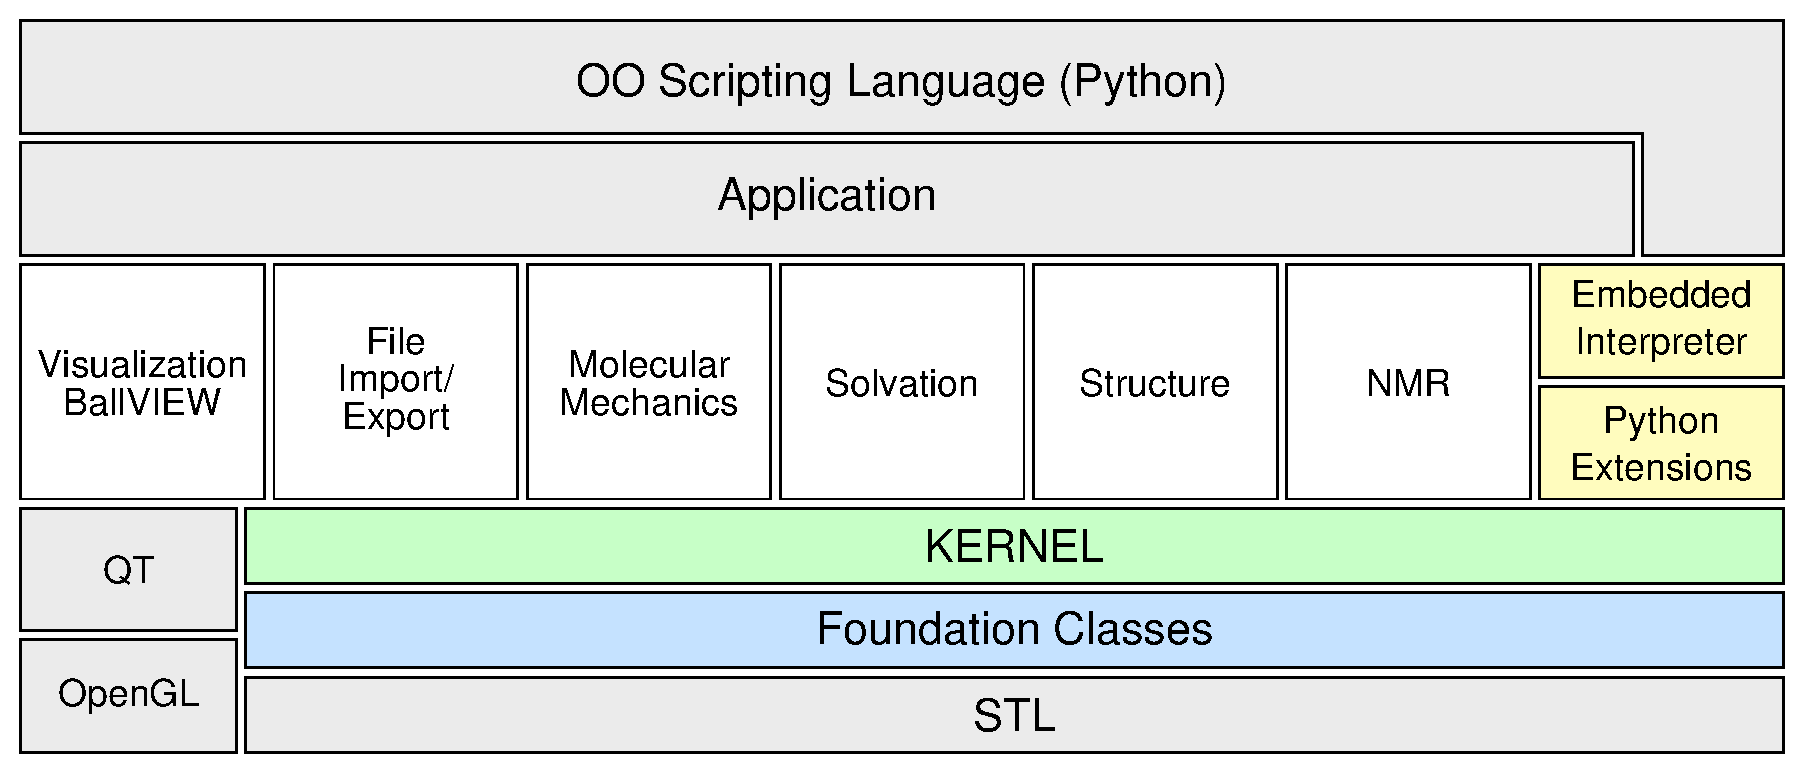
\includegraphics[width=\textwidth]{BALL_structure.eps}
  \caption{Overview of the structure of BALL}
  \label{fig:BALL_structure}
\end{figure}

The third layer of classes (on top of the foundation classes and the kernel)
provides the functionality required for applications. We call them
\newterm{basic components}. Each of these basic components is independent of
the other components.  We have implemented five basic components that cover
\Index{Molecular Mechanics}, file import/export, advanced \Index{solvation
methods}, structure analysis/comparison and \Index{visualization}. These
areas were selected, because our main interest stems from the field of protein
docking. The Molecular Mechanics component does not only provide standard
force fields (AMBER~\cite{AMBER95}, CHARMM~\cite{BBO+83}), but also a generic
\Index{force field}.  This generic force field is a base class for all force
fields. It implements fundamental methods to manage parameter files, parameter
assignment, and atom type assignment, and defines a common interface for all
force fields. Thus, large portions of code may be reused for the
implementation of new force fields.  The file import/export component
implements general methods for efficient file handling, but also methods to
read and write the most common file formats used for molecular structures
(\eg, PDB, MOL2). The solvation component provides methods for calculating
solvation effects. The first method that accounts for solvation is the atomic
contact energy by Zhang {\it et al.}~\cite{ZVC+97}. The second approach that
we implemented is a numerical solver for the \Index{Poisson-Boltzmann} equation.  The
structure component contains algorithms to search for common structural motifs
in proteins, to map molecules onto each other, and to calculate solvent
accessible and solvent excluded surfaces of molecules. For the visualization
of the results, we designed \Index{VIEW}, a class hierarchy that
visualizes BALL kernel objects with standard representations (ball and stick,
van der Waals, ribbons, surfaces, \etc). The visualization was implemented
using OpenGL and QT~\cite{QT}. Hence, it is highly portable and enables the
user to produce state-of-the-art graphical user interfaces with a minimum
effort.

The fourth layer in BALL consistes of Python bindings. Python is an
object-oriented scripting language that is easy to learn and very readable.
BALL provides Python bindings for most of its classes, which allow the use of
the BALL \CPP classes from Python. This approach drastically reduces the
turn-around times (no compiling and linking phase is required) and adds
scripting capabilities to BALL without introducing a new and exotic scripting
language. The Python bindings use the same class names as the BALL classes,
therefore after the initial rapid development of a methodology, the existing
Python code can be easily ported back to \CPP for production purposes.
Chapter \ref{chapter:python} gives a short introduction to this feature.



\chapter{Getting Started}
\label{chapter:getting-started}
\section{System Requirements}

\subsection{Compiler}
\index{compiler}
  BALL requires a (more or less) ANSI compliant \CPP compiler.
  It has been successfully built and tested on the following platforms:
	\begin{itemize}	
   	\item Linux/x86 2.x using g{\tt ++} 3.3.3
%   	\item Linux/x86 2.x using g{\tt ++} 2.95.3
%   	\item Linux/x86 2.x using Kuck \& Associate (KAI) \CPP 4.0
   	\item Linux/x86 2.x using Intel C++ Compiler 8.0
   	\item Solaris/SPARC 8 using g{\tt ++} 3.2.1
%   	\item Solaris/SPARC 8 using g{\tt ++} 2.95.3
%   	\item Solaris/SPARC 8 using Kuck \& Associate (KAI) \CPP 4.0
%   	\item Solaris/SPARC 8 using Sun Forte Developer 7 C{\tt ++} 5.4 2002/03/09
   	\item IRIX 6.5 using CC 7.3.1.1m (32 and 64 bit)
%   	\item Compaq Tru64 Unix V4.0f using Compaq \CPP 6.3
		\item Microsoft Windows XP using Microsoft Visual Studio .NET (MSVC 7.0) and Visual Studio Express 2005
 	\end{itemize}

\subsection{BALL on the Windows platform}
For instructions on how to install BALL on the Windows platform, please
have a look at BALL/Windows/README.txt . The sections below will describe
how to build BALL on Unix, Linux and MacOS...

\subsection{External software and libraries}
BALL needs {\tt flex} and {\tt bison} for automatically generating parsers
for various purposes. These utilities are standard software and should be
installed on every contemporary UN*X machine. The newest versions are
downloadable from \URL{http://www.gnu.org/software/}.

The usage of GNU {\tt make} is recommended, although BALL will also build with
other versions of {\tt make}. It is available from \URL{ftp://ftp.gnu.org/gnu/}
and easy to install.

The compilation of the visualization component VIEW also requires
the QT library (at least version 3.2), which is available from
\URL{www.trolltech.com/products/qt}/.

If QT was not installed in one of the standard library paths or the
QT header files were not installed in one of the compiler's default
include directories, use \mbox{"\option{--with-qt-libs}{\tt{}=DIR}"} and
\mbox{"\option{--with-qt-incl}{\tt{}=DIR}"} as options to configure (see
Section \ref{section:building-ball}) to specify the paths QT was installed
to.\index{QT} {\tt configure} will also honor the {\tt QTDIR} environment variable.

QT also requires OpenGL. On platforms that do not provide OpenGL, Mesa can
be used. Mesa is a 3-D graphics library with an API which is 
very similar to that of OpenGL. It can be obtained from 
\URL{http://www.mesa3d.org}.
\index{MESA}

If your machine has a graphics accelerator from ATI oder NVidia, 
you can use the vendor-provided OpenGL drivers (\URL{http://www.ati.com/support/driver.html}
and \URL{http://www.nvidia.com/object/linux.html}).
But be warned, we experienced serious trouble with both of the drivers. They
still seem to be unstable up to now (February 2004). If you have freezes in
BALLView or display problems in the 3D view, please have a look at our FAQ
which addresses some of the issues
(\URL{http://www.ball-project.org/Support/FAQ}).

To use the Python extensions of BALL (Python is an object oriented
scripting language), you will also need Python (version 2.2 or above) installed
(\URL{http://www.python.org}) and a recent version of SIP (version 4.0rc2 or
above, available at \URL{http://www.riverbankcomputing.co.uk/sip/}). SIP is a tool
for generating Python bindings for C++ class libraries.

Additionally you might need the FFTW package for fast Fourier
transformations (Verson 2.1.3), available from \URL{http://www.fftw.org/}.

Please make sure that the required external \CPP libraries (i.e. QT and SIP)
have been compiled with the same compiler (and compiler version!) as the BALL
libraries. Otherwise you will most likely see a plethora of strange error
messages, either while linking applications or at runtime.

\section{Installation}
\label{section:building-ball}

Building BALL is very easy, but please read through this section carefully to
avoid any problems.  If all requirements stated above are met, BALL is built
by issuing the following commands in the directory {\tt BALL/source}:

\begin{lstlisting}{}
  ./configure
  make
\end{lstlisting}

The following sections give further details on the configuration of the library,
on the library files created, how to test the library, and how to build BALL 
applications.

\subsection{Configuring BALL}
\index{configure!usage}

"{\tt configure}" tries to gather as much information on your system as possible and 
then creates the necessary configuration files (\file{config.h},
\file{config.mak}, \file{common.mak}, and \file{Makefile}).
The configuration of BALL may be adapted to your needs and to your system
configuration from the command line by adding one or more of the options from
Table \ref{table:options}.
An overview of these options can also be obtained by executing "{\tt configure
--help}"

% \begin{center}
\begin{longtable}{lp{7cm}}\hline
  \option{--x-includes}{\tt{}=DIR}&        X include files are in DIR\\\vspace{3mm}

  \option{--x-libraries}{\tt{}=DIR}&       X library files are in DIR\\\vspace{3mm}

  \option{--enable-optimization}&          optimize the library for speed, remove debug info\\\vspace{3mm}

  \option{--enable-debuginfo}&             create debug information\\\vspace{3mm}

  \option{--disable-VIEW}&                 disable the compilation of the visualization
                                           classes\\\vspace{3mm}

  \option{--enable-64}&                    build 64 bit objects (if allowed
                                           by the compiler)\\\vspace{3mm}

  \option{--with-compiler}{\tt{}=CXX}& use CXX to compile BALL\\\vspace{3mm}

  \option{--with-cxxflags}{\tt{}=FLAGS}&   add FLAGS to the \CPP compiler flags
                                           (commas are converted to blanks)
                                           \\\vspace{3mm}

  \option{--with-ldflags}{\tt{}=FLAGS}&    add FLAGS to the linker flags
                                           (commas are converted to blanks)
                                           \\\vspace{3mm}

  \option{--with-arflags}{\tt{}=FLAGS}&    add FLAGS to the flags for the
                                           creation of the static libraries
                                           \\\vspace{3mm}

  \option{--with-dynarflags}{\tt{}=FLAGS}& add FLAGS to the flags for the
                                           creation of the shared libraries
                                           \\\vspace{3mm}

	\option{--with-qt}{\tt{}=QTDIR}& QT installation is in QTDIR. This option 
																						is equivalent to setting the {\tt
																						QTDIR} environment variable.
																						Using this option should be
																						preferred over the next two
																						options, which are only necessary
																						if the QT installation has non-standard paths for libraries and headers.\\
																					\vspace{3mm}
  \option{--with-qt-incl}{\tt{}=DIR}&      QT header files are in DIR\\
                                           \vspace{3mm}

  \option{--with-qt-libs}{\tt{}=DIR}&      QT libraries are in DIR\\\vspace{3mm}
	\option{--with-qt-mt}&										Use the multithreaded version of the QT
																						libraries rather than the singlethreaded 
																						one (libqt-mt instead of
libqt).
																						\\\vspace{3mm}
	\option{--with-moc}{\tt{}=MOC}& 					The absolute path to the QT meta object
																						compiler (moc, typically found in
																						{\tt\$QTDIR/bin/moc})\\\vspace{3mm}

	\option{--with-uic}{\tt{}=UIC}& 					The absolute path to the QT user interface
																						compiler (uic, typically found in
																						{\tt\$QTDIR/bin/uic})\\\vspace{3mm}

  \option{--with-opengl-incl}{\tt{}=DIR}&  OpenGL/Mesa header files are in DIR/GL\\\vspace{3mm}

  \option{--with-opengl-libs}{\tt{}=DIR}&  OpenGL/Mesa libraries are in DIR/GL\\\vspace{3mm}

  \option{--with-mesa}&                    use MESA instead of OpenGL\\
                                           \vspace{3mm}

  \option{--without-libxnet}&              use \Index{libsocket}/\Index{libnsl}
                                           for linking rather than 
                                           \Index{libxnet} (under Solaris)
                                           \\\vspace{3mm}

  \option{--with-python=EXE}& 							Enable Python support using the
																						Python executable in EXE. If no
executable is specified ({\tt --with-python} only), {\tt configure} looks for
an installed python in the current PATH.
																						Typically, from the executable {\tt configure} can figure out where the
																						headers and the library are hidden, so that the following two options are
																						usually not required.\\\vspace{3mm}
  
  \option{--with-python-incl=DIR}&         Python includes (Python.h) is in
                                           DIR\\\vspace{3mm}

  \option{--with-python-libs=DIR}&         Python library (libpython*.a) is
                                           in DIR\\\vspace{3mm}

  \option{--with-python-ldopts=X}&         Use additional options X when
                                           linking with the Python library
                                           \\\vspace{3mm}

  \option{--with-sip-lib}{\tt{}=DIR}&             the SIP library resides in DIR
                                           \\\vspace{3mm}

  \option{--with-sip-incl}{\tt{}=DIR}&            the SIP header file resides in DIR
                                           \\\vspace{3mm}

  \option{--with-sip}{\tt{}=DIR}&                 the SIP executable resides in DIR
                                           \\\vspace{3mm}

  \option{--without-xdr}&                  no RPC/XDR headers available - do
                                           not build portable binary
                                           persistence support
                                           \\\vspace{3mm}
	\option{--with-fftw-lib}{\tt{}=DIR}& Enable support for the FFTW library and
																				search for the library in {\tt DIR}.
																					\\\vspace{3mm}
	\option{--with-fftw-incl}{\tt{}=DIR}& 	Header files for FFTW are in {\tt DIR}.
																					Required for non-standard include
																					paths only.
																					\\\vspace{3mm}

  \option{--help}&                         display help information\\\hline
\caption{options for {\tt configure}}
\label{table:options}
\end{longtable}
%\end{center}
%\caption{options for {\tt configure}}
%\label{table:options}

For example, to compile BALL without the visualization component,
specify 
\begin{lstlisting}{}
  configure --disable-VIEW
\end{lstlisting}

To compile the visualization classes using the QT installation in
/opt/misc/qt, specify the path to the QT directory as follows:

\begin{lstlisting}{}
  configure --with-qt=/opt/misc/qt
\end{lstlisting}


If the headers or libraries are installed in non-standard directories, you can
also specify them separately:

\begin{lstlisting}{}
  configure --with-qt-libs=/opt/lib 
		--with-qt-incl=/opt/qt/include
\end{lstlisting}

If Mesa should be used (when compiling under Linux), the correct options might look
like this:

\begin{lstlisting}{}	
  configure --with-qt-libs=/opt/qt/lib 
		--with-qt-incl=/opt/qt/include
    --with-opengl-libs=/opt/mesa/lib 
		--with-opengl-incl=/opt/mesa/include
\end{lstlisting}

\subsection{Building the Libraries}

After the successful termination of configure, issuing "make" will build the
shared libraries. Two different libraries will be built:

\begin{center}
	\begin{tabular}{ll}
  	\file{libBALL.so}&     the main BALL library\\
  	\file{libVIEW.so}&     the visualization classes\\
	\end{tabular}
\end{center}

The latter library is not built if "\option{--disable-VIEW}" is specified or configure
cannot find X libraries, OpenGL libraries, or QT libraries (and the respective headers).

It is also possible (although not recommended) to build the corresponding static libraries
\file{libBALL.a} and \file{libVIEW.a} using "{\tt make
staticlibs}". Please note that statically linked binaries are huge.

\subsection{Installing the Libraries}

After compiling the libraries, they are installed in {\tt BALL/lib/\${BINFMT}/}
when calling "{\tt make install}" where {\tt \${BINFMT}} is the binary format
as determined by {\tt configure}.  Currently, the only way to install the
libraries somewhere else is by moving them by hand to the desired destination.
Wherever you install the shared libraries, please make sure to include their
location in the \Index{{\tt LD\_LIBRARY\_PATH}} environment variable.

If you are using \Index{csh}, \Index{tcsh}, or similar shells, use the command
\begin{lstlisting}{}
   setenv LD_LIBRARY_PATH DIR
\end{lstlisting}

\noindent to set the library path. If you are using \Index{sh}, \Index{bash},
or related shells, try

\begin{lstlisting}{}   
   LD_LIBRARY_PATH=DIR
   export LD_LIBRARY_PATH
\end{lstlisting}

If you installed the shared libraries in a directory that the dynamic linker
\Index{ld} searches by default, it is not necessary to set {\tt
LD\_LIBRARY\_PATH}.

\section{Testing the Library}
\index{testing}
\index{test programs}

\subsection{Unit tests}

BALL provides an extensive suite of test programs to ensure the correctness of
the code on all platforms. This test suite requires a lot of patience since
the compilation takes quite some time. However, we recommend to run these
tests to ensure that the library is fully operational. At the moment, the test
suite does not yet cover all functionality of BALL, but only some chosen
classes.  The test programs are located in the directory {\tt
BALL/source/TEST}.  To compile and run the test suite, use "{\tt make test}".
Please make sure that {\tt LD\_LIBRARY\_PATH} is correctly set, otherwise the
execution of the test programs will fail.

Each of the test programs tests one or more classes of BALL. When a test
program (\eg~{\tt Atom\_test}) is run, the program prints either "OK" (if all
tests passed) or "FAILED" if any of the tests failed. "{\tt make test}" runs
all tests and complains if a certain test fails.  


If this happens, please let report a bug through our online bug tracking
system at \URL{http://www.ball-project.org/Support/BugTracker}.

\noindent
For all bug reports, please include your system configuration, the file
\file{config.log} (which contains the results of tests configure performed),
and the file \file{BALL/include/BALL/config.h} (which contains the compiler
defines used by BALL).

\subsection{Benchmarks}

If you want to know how fast the version of BALL is compared to other systems,
you might want to run the benchmark suite in \directory{BALL/source/BENCHMARKS}.
You can compile the benchmark suite by changing to that directory and running
"{\tt make}". After that, run the benchmarks with "{\tt make bench}".
Depending on your hardware and whether you compiled BALL with or without
optimization, running the benchmarks will take up to several minutes. Upon
termination, it will print an overall number, the BALLStones. This number is a
crude estimate of the performance you can expect for a mix of typical BALL
applications. The benchmark suite currently includes benchmarks for the BALL
kernel data structures, file I/O, the AMBER force field, and the
Poisson-Boltzmann solver. The BALL web site contains a list of benchmark
results for different platforms, please feel free to submit your results for
inclusion.

\include{building-python}

\chapter{First Steps With BALL}
\label{chapter:first-steps}
\section{Building molecules}

Since BALL is intended for Molecular Modeling, the classes representing atoms,
bonds, and molecules are of central importance. In this first example, we will
construct a water molecule ``by hand'' to illustrate the use of these classes.
Typical applications would read molecular structures from a file. This will be
shown in the second example.

\noindent
To start the construction of a water molecule, we first create an (empty)
\Index{atom}. Atoms are represented by the class \class{Atom}.

\begin{lstlisting}{}
	Atom* oxygen = new Atom;
\end{lstlisting}
	
\noindent
Atoms have a number of attributes. As we created this atom without specifying
any of its properties, these attributes are set to their defaults. The
following table lists the attributes of an atom along with its
\newtermdef{accessors} (methods to access or modify an attribute) and default
values.
\begin{center}
	\begin{tabular}{lllc}
	attribute		&	type				& accessors     						& default\\
	\hline
	name				& String			& setName,getName						& {\tt ""}\\
	element			& Element			& setElement,getElement			& {\tt Element::UNKNOWN}\\
	charge			& float				& setCharge,getCharge				& 0.0\\
	radius			& float				& setRadius,getRadius				& 0.0\\
	type name   & String			& setTypeName,getTypeName		& {\tt ""}\\
	type        & Atom::Type	& setType,getType						& {\tt Atom::INVALID\_TYPE}\\
	position    & Vector3			& setPosition,getPosition		& (0, 0, 0)\\
	velocity    & Vector3			& setVelocity,getVelocity		& (0, 0, 0)\\
	force		    & Vector3			& setForce,getForce					& (0, 0, 0)
	\end{tabular}
\end{center}

\noindent
For example, we can assign the \Index{element} for our new atom:

\begin{lstlisting}{}
	oxygen->setElement(PTE[Element::O]);
\end{lstlisting}

\noindent
The expression {\tt PTE[\class{Element}::O]} returns an instance of class
\class{Element}. It is assigned to our atom using the \method{setElement}
method. We leave our new atom at the default position (0, 0, 0) and create two
new atoms, which will be the still missing hydrogen atoms:

\begin{lstlisting}{}
	Atom* hydrogen1 = new Atom;
	Atom* hydrogen2 = new Atom;
	hydrogen1->setElement(PTE[Element::H]);
	hydrogen2->setElement(PTE[Element::H]);
\end{lstlisting}
	
\noindent
Now we have to assign the correct coordinates to the two hydrogen atoms.  The
method \method{setPosition} takes an instance of \class{Vector3} as an
argument. This class is used to represent coordinates and vectors in
three--dimensional space. An object of type \class{Vector3} can be constructed
from three floating point numbers which represent the x, y, and z coordinates.
Thus, we can assign the coordinates as follows:
 
\begin{lstlisting}{}
 	hydrogen1->setPosition(Vector3(-0.95, 0.00, 0.0));
 	hydrogen2->setPosition(Vector3( 0.25, 0.87, 0.0));
\end{lstlisting}

\noindent

Now, our three atoms are of the right type and at the right positions. However, we
do not yet have a molecule, so let's create one:\\

\begin{lstlisting}{}
	Molecule* water = new Molecule;
\end{lstlisting}

\noindent
Molecules are representd by the \class{Molecule} class. Each instance of this
class may contain an arbitrary number of atoms. Using the \method{insert}
method, we can construct a molecule from our atoms:

\begin{lstlisting}{}
	water->insert(*oxygen);
	water->insert(*hydrogen1);
	water->insert(*hydrogen2);
\end{lstlisting}

\noindent
For a complete water molecule, we still need two \Index{bonds}. This can be
achieved with the method \method{createBond}:
	
\begin{lstlisting}{}
	oxygen->createBond(*hydrogen1);
	oxygen->createBond(*hydrogen2);
\end{lstlisting}

or

\begin{lstlisting}{}
	hydrogen2->createBond(*oxygen);
\end{lstlisting}

\noindent
To verify that everything worked as expected, we might print the number of
atoms in the molecule or the number of bonds for each atom:
	
\begin{lstlisting}{}
	cout << "# of atoms in water: " 
 			 << water->countAtoms() << endl;
	cout << "# of bonds of oxygen: " 
			 << oxygen->countBonds() << endl;
	cout << "# of bonds of hydrogen1: " 
		   << hydrogen1->countBonds() << endl;
	cout << "# of bonds of hydrogen2: " 
			 << hydrogen2->countBonds() << endl;
\end{lstlisting}

\noindent
The method \method{countAtoms} is available for all kernel classes that might
contain atoms and returns the total number of atoms for this object. The
method \method{countBonds} returns the number of bonds the atom shares. An
atom can have at most eight bonds.

We can also verify the bond distances:
\begin{lstlisting}{}
	Vector3 bond_vector = oxygen->getPosition() 
										    - hydrogen1->getPosition();

	cout << "bond distance: " 
			 << bond_vector.getLength() << endl;
\end{lstlisting}
	
\noindent
\method{getPosition} is the complementary method of \method{setPosition}: it
returns the current position of an atom. The return value is again of type
\class{Vector3}. The length of this vector is then returned by the
\method{getLength} method. 

Water molecules rarely occur alone, so we are going to create further water molecules.
All BALL kernel classes are container classes and support \newterm{deep
copying}, \ie when assigned or copy constructed their contents are copied as
well. So, we can easily create a new water molecule:

\begin{lstlisting}{}
	Molecule* water2 = new Molecule(*water);
\end{lstlisting}
	
\noindent
This molecule is an exact copy of our original water molecule. Especially, the
atoms have the same position as in the original. So we want to shift the whole
molecule to another position.  In principle, we could access all atoms in the
copy and add a constant translation vector to their position. However, there
is a simpler way. BALL provides so--called \newterm{processors}. These
processors may be applied to any of the kernel objects and perform an
operation on any objects they encounter. For example the
\class{TranslationProcessor} performs a simple translation on every atom it
finds. The use of the processors is very simple.  All kernel classes define an
\method{apply} method wich takes a processor as an argument. In order to
translate our second water molecule by a certain distance, we first create a
\class{TranslationProcessor}:

\begin{lstlisting}{}
	TranslationProcessor translation(Vector3(5, 0, 0));
\end{lstlisting}
	
\noindent
The translation vector is specified as the argument of the constructor. Now we
may translate the atoms of our water molecule by a simple call to \method{apply}

\begin{lstlisting}{}
	water2->apply(translation);
\end{lstlisting}

\noindent
Another important kernel class besides atoms and molecules is \class{System}.
A system is a collection of atoms, molecules, or any other kernel objects. For
example, we can store our two water molecules in a system object:

\begin{lstlisting}{}
	System S;
	S.insert(*water);
	S.insert(*water2);
\end{lstlisting}

\begin{figure}[t]
	\centering
	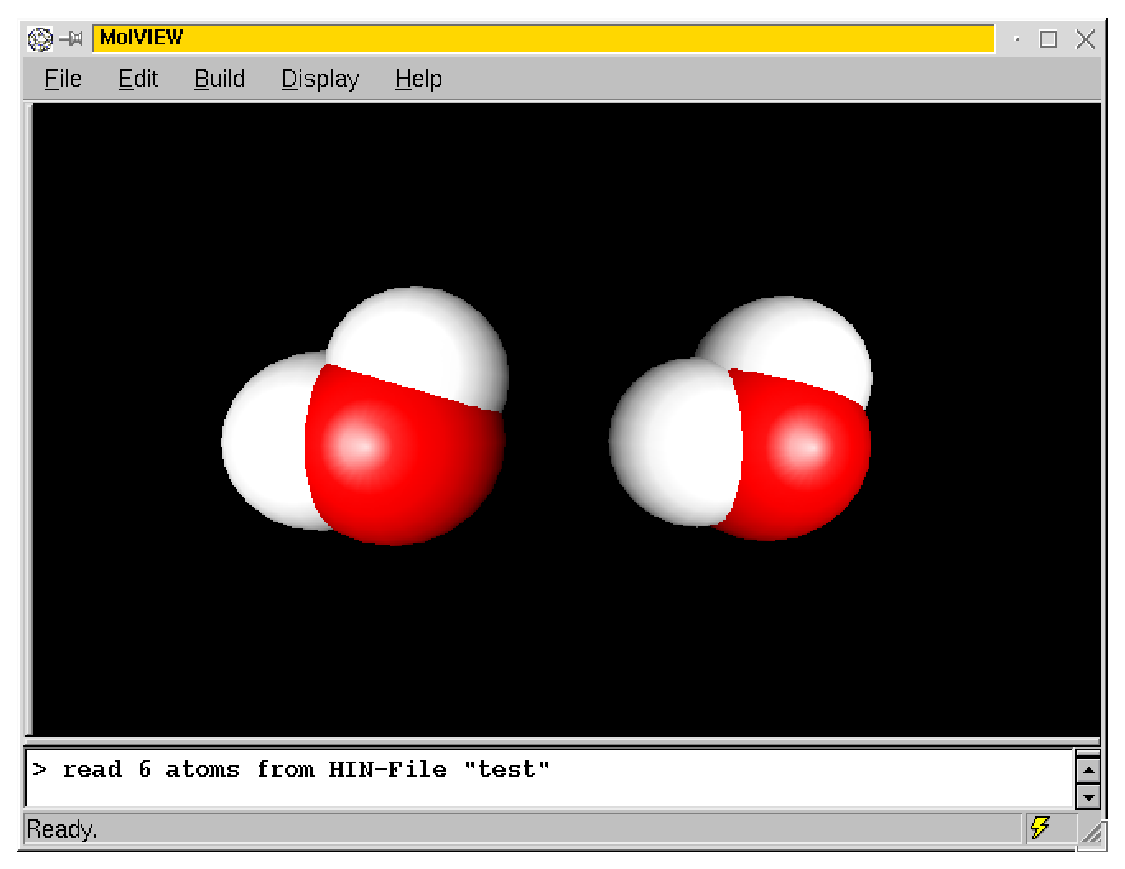
\includegraphics[width=\textwidth]{tut1_screenshot}
	\caption{Screenshot of BALLView showing the result of the first example
					 ({\tt tutorial1.C})}
	\label{fig:tut1-screenshot}
\end{figure}
\noindent
We can now manipulate the two water molecules simultaneously. For example a
further application of the translation processor to the system would apply
the translation to both molecules.
But now we would like to have a look at what we built. So we might write our
system to a file and inspect it with a molecule viewer (\eg BALLView).
BALL supports a variety of file formats. For example we could write the system
to a HyperChem HIN file~\cite{HyperChem}:
\begin{lstlisting}{}
	HINFile outfile("water.hin", File::OUT);
	outfile << S;
	outfile.close();
\end{lstlisting}
\noindent
These three lines of code create a \class{HINFile} object which is used to
read and write HyperChem files. The first line opens a file named {\tt
water.hin} for output ({\tt File::OUT}; if the second argument is omitted the
file is opened for reading only).
The second line uses the stream operator {\tt <<} to write the contents
of system {\tt S} to this file. The file is closed in the third line.

% ????? [anker]
% The following is not true. If we use a pointer here, then it's OK, but
% with a System it simply doesn't work. What do we want here? I'd prefer a
% Sytsem instead of a System*.

% Finally, we have to delete all the objects we created. This is very simple:
% 
% \begin{lstlisting}{}
% 	delete S;
% \end{lstlisting}

\noindent 
As all molecules and atoms we created are inside the system, they are deleted
automatically as soon as the system is deleted.

If this short program is run it creates the following output:

\begin{lstlisting}[frameround=]{}
	# of atoms in water: 3
	# of bonds of oxygen: 2
	# of bonds of hydrogen1: 1
	# of bonds of hydrogen2: 1
	bond distance: 0.95
\end{lstlisting}

\noindent
It also creates a file named {\tt water.hin} which contains the two water
molecules. Fig.~\ref{fig:tut1-screenshot} shows the contents of this file
in the BALLView viewer.

To compile this small example, we still have to include a few header files.
The complete file is shown in Listing~\ref{lst:tutorial1} on
page~\pageref{lst:tutorial1} and can be found in \mbox{{\tt
BALL/source/TUTORIAL/tutorial1.C}}.

First, we have to include \file{iostream} as we use {\tt cout} and {\tt endl}
to print some text. Then, we have to include the headers for the BALL kernel
classes \class{Atom}, \class{Bond}, \class{Molecule}, \class{System}, and
\class{PTE}. The headers for the HyperChem file support are found in the
directory \directory{BALL/FORMAT} and the headers for the
\class{TranslationProcessor} class are found in
{\tt BALL/STRUCTURE/geometricProperties.h}.

As all BALL classes are hidden in the \namespace{BALL} namespace, we have to
give access to this namespace with the command 
\begin{lstlisting}{}
	using namespace BALL;
\end{lstlisting}
Similarly, we also use the namespace \namespace{std} which contains {\tt cout}
and {\tt endl}.

If you have BALL installed, you might now try to compile this example. Simply
change to the directory \directory{BALL/source/TUTORIAL} which contains all
the examples from this tutorial and type 
\begin{lstlisting}[frameround=]{}
	make tutorial1
	./tutorial
\end{lstlisting}
This should build and execute the example. Please remember to set the
environment variable {\tt LD\_LIBRARY\_PATH} to the directory where your
libraries are installed.

After the successful execution of the example, a file named {\tt water.hin}
should appear in the current directory. This file contains the two water
molecules. You might inspect it with the molecule viewer BALLView.
Fig.~\ref{fig:tut1-screenshot} shows a screenshot of BALLView displaying the two
water molecules.

\newpage
\begin{lstlisting}[captionpos=t,caption={The complete source code of the first example.}\label{lst:tutorial1}]{}
// tutorial example 1
// ------------------
// build two water molecules and write them to a file

// needed for cout
#include <iostream>

// the BALL kernel classes
#include <BALL/KERNEL/atom.h>
#include <BALL/KERNEL/bond.h>
#include <BALL/KERNEL/molecule.h>
#include <BALL/KERNEL/system.h>
#include <BALL/KERNEL/PTE.h>

// reading and writing of HyperChem files
#include <BALL/FORMAT/HINFile.h>

// the TranslationProcessor
#include <BALL/STRUCTURE/geometricTransformations.h>

// we use the BALL namespace and the std namespace
using namespace BALL;
using namespace std;

int main()
{
	// we create a new atom called oxygen
	// and set its element to oxygen (PTE[Element::O])
	Atom* oxygen = new Atom;
	oxygen->setElement(PTE[Element::O]);

	// now we create two hydrogen atoms...
	Atom* hydrogen1 = new Atom;
	Atom* hydrogen2 = new Atom;
	hydrogen1->setElement(PTE[Element::H]);
	hydrogen2->setElement(PTE[Element::H]);

	// ...and move them to approximately correct positions
 	hydrogen1->setPosition(Vector3(-0.95, 0.00, 0.0));
 	hydrogen2->setPosition(Vector3( 0.25, 0.87, 0.0));

	// We create our water molecule...
	Molecule* water = new Molecule;

	// ...and insert the three atoms into the molecule.
	water->insert(*oxygen);
	water->insert(*hydrogen1);
	water->insert(*hydrogen2);

	// Then we build the two O-H bonds
	oxygen->createBond(*hydrogen1);
	oxygen->createBond(*hydrogen2);

	// Some statistics: Molecule::countAtoms() 
	// returns the number of atoms, Atom::countBonds() 
	// the number of bonds the atom shares
	cout << "# of atoms in water: " 
			 << water->countAtoms() << endl;
	cout << "# of bonds in oxygen: " 
			 << oxygen->countBonds() << endl;
	cout << "# of bonds of hydrogen1: " 
			 << hydrogen1->countBonds() << endl;
	cout << "# of bonds of hydrogen2: " 
			 << hydrogen2->countBonds() << endl;

	// bond_vector is a vector and is set to the
	// difference of atom positions of oxygen and hydrogen1
	Vector3 bond_vector = oxygen->getPosition() 
											- hydrogen1->getPosition();

	// Vector3::getLength: the length of the vector
	cout << "bond distance: " 
			 << bond_vector.getLength() << endl;

	// Now we copy our molecule using a copy constructor.
	Molecule* water2 = new Molecule(*water);

	// A translation processor moves the second molecule
	// 5 Angstrom along the x axis
	TranslationProcessor translation(Vector3(5, 0, 0));
	water2->apply(translation);

	// We insert our two molecules into a system
	System* S = new System;
	S->insert(*water);
	S->insert(*water2);

	// and write this system to a HyperChem file
	HINFile outfile("water.hin", File::OUT);
	outfile << *S;
	outfile.close();

	// We delete the system. This also deletes 
	// the molecules and the atoms therein
	delete S;
}
\end{lstlisting}

\section{Handling proteins}

In the second example we take a step towards real world applications. Instead
of constructing our own molecules, we now read a protein from a \newterm{PDB
file}. The PDB format~\cite{PDB} is a standardized file format for molecular structure
data. In our case, we will read BPTI (bovine pancreatic trypsin inhibitor), a
small protein:

\begin{lstlisting}{}
	PDBFile infile("bpti.pdb");
	System S;
	infile >> S;
	infile.close();
\end{lstlisting}

\noindent
In the first line, we create a \class{PDBFile} object and assign it to a file
named {\tt bpti.pdb}. Then we create an empty system {\tt S} and read the
contents of the PDB file into the system using the stream operator {\tt >>}.
This use of the stream operators is possible for all file formats in BALL (see
also the first example). Hence, you can easily switch file formats
by changing just the type of the {\tt infile} object (\eg replace it by
\class{HINFile} to read HyperChem files).

We can now verify whether the file was correctly read. BPTI should have 454
atoms. As mentioned before, for each kernel object containing atoms
(\ie classes that are derived from \class{AtomContainer}), we can obtain the
actual number of atoms by calling \method{countAtoms}:

\begin{lstlisting}{}
	cout << "# of atoms in BPTI: " << S.countAtoms() << endl;
\end{lstlisting}

Now, we are interested in the sequence of BPTI. Since BPTI contains only a
single chain, we might just traverse all residues of this chain and write
their names to {\tt cout}. This is done by \newterm{iterators}. Iterators are
objects that can be used to traverse container objects (\eg lists, arrays, or
-- in our case -- proteins). Iterators ``point'' to an element of a container
object. They may be incremented to get the next element and they may be
dereferenced similar to pointers by using {\tt *} or {\tt ->}. In fact,
C pointers can be thought of as iterators.
The use of iterators in BALL is similar to the
use of iterators in the \newterm{Standard Template Library} (\Index{STL}).
But there is a significant difference. STL containers usually contain objects of
one single type (\eg a list of strings). In BALL kernel objects, this is
different. A system may contain atoms, proteins, molecules, residues, \etc
This leads to a difference in the interface. A typical {\tt for} loop using STL
iterators to access all elements of a list looks as follows:

\begin{lstlisting}{}
	list<string> string_list = ...;
	list<string>::iterator list_it;
	
	for (list_it = string_list.begin(); 
			 list_it != string_list.end();
			 ++list_it)
	{
		cout << *list_it << endl;
	}
\end{lstlisting}

\noindent
Here, we use a list iterator ({\tt list\_it}) to traverse the whole list ({\tt
string\_list}). The method {\tt begin()} returns an iterator that points to
the first element of the list. In the {\tt for} loop we increment the iterator
until it equals the iterator returned by {\tt end()}. This method returns a
past--the--end iterator, \ie the iterator points beyond the last element of
the container. In the body of the {\tt for} loop, we access the list element
the iterator points to using the {\tt *} operator.

Traversing a BALL kernel data structure is as simple as traversing a list with
STL. But since kernel objects may contain objects of a variety of types,
we have to define over which objects we intend to iterate.
For example iterating over all residues of our system requires a
\class{ResidueIterator}. Clearly, we also need different {\tt begin()} and
{\tt end()} methods for all data types. Hence, the loop that prints the
sequence of our protein reads as follows:

\begin{lstlisting}{}
	ResidueIterator res_it;
	for (res_it = S.beginResidue(); 
			 res_it != S.endResidue();
			 ++res_it)
	{
		cout << res_it->getName() << " ";
	}
	cout << endl;
\end{lstlisting}

\noindent
This loop iterates over all residues in {\tt S} and uses the method {\tt
Residue::}\method{getName()} to access the residues name. All proteins and
residues are traversed in the order in which they appear in the PDB file.
Since the PDB format requires the residues to start with the N-terminus,
the sequence is printed  in the correct order (N-terminus to C-terminus). 

\noindent
The source code for this example can be as {\tt tutorial2.C} found in
\directory{BALL/source/TUTORIAL}.

\section{A simple AMBER calculation}

\index{Energy minimization}
\index{optimizing hydrogens}

Having introduced the basics of handling proteins in the last chapter, we now
turn towards real-life examples: performing a molecular dynamics simulation
with a protein structure from PDB. Again, we will be using BPTI, reading it
from a PDB file as in the previous example:

\begin{lstlisting}{}
	PDBFile	infile("pdb4pti.ent");
	System S;
	infile >> S;
	infile.close();
\end{lstlisting}

\noindent
The file we chose to read here is the original file as obtained from
the PDB, therefore it contains neither hydrogen atoms, nor bonds.
The BALL class \class{FragmentDB} provides a convenient way to solve
both problems. \class{FragmentDB} is an extendible database of residue
structures. By comparing the residues in the PDB file with the reference
templates in the \class{FragmentDB}, we can identify the missing bonds
and hydrogen atoms. A matching between atoms is computed based on the names,
so the atom names have to adhere to the PDB naming convention.
For deviating naming schemes, \class{FragmentDB} provides a member instance
\member{}{normalize\_names}, which tries to convert the names to the PDB 
naming convention. \member{}{normalize\_names} is a processor, so we
can \member{Composite}{apply} it to any given kernel data structure:

\begin{lstlisting}{}
	FragmentDB db("fragments/Fragments.db");
	S.apply(db.normalize_names);
\end{lstlisting}

\noindent
Instantiating \class{FragmentDB} usually takes a few seconds to parse the
fragment database and the naming conversion tables stored in
\directory{BALL/data/Fragments}. The resulting data may then be used by two
very handy processors: add\_hydrogens and build\_bonds.
As their names suggest, those processors add the missing hydrogen atoms and
rebuild missing bonds. We will now add the missing atoms and bonds of BPTI 
through simple application of the two processors:

\begin{lstlisting}{}
	S.apply(db.add_hydrogens);
	S.apply(db.build_bonds);
\end{lstlisting}
\index{adding hydrogens}
\index{building bonds}

\noindent
Now we have constructed a complete protein structure of BPTI. We can verify
this by applying a \class{ResidueChecker} to the system.
\class{ResidueChecker} is a processor that performs a number of consistency
checks on a given kernel data structure:
\begin{itemize}
	\item check for missing atoms
	\item check for overlapping atoms (closer than 0.5 \AA)
	\item check for integrality of residue charges (not relevant here)
	\item check bond lengths (should be within 15\% of the template bond lengths)
\end{itemize}
The information on missing atoms and bond lengths is taken from an instance
of \class{FragmentDB}:\index{fragment database}

\begin{lstlisting}{}
	ResidueChecker rc(db);
	S.apply(rc);
\end{lstlisting}
\index{checking residues}
	
\noindent
If the \class{ResidueChecker} notices a problem with the structure, it will 
print a warning. In our case, it was (hopefully) correct, so nothing will
happen.

Although our protein structure is correct, the positions of the added hydrogen
atoms are only approximations of the true positions.
\class{AddHydrogensProcessor} tries to set the positions based on the
positions given in the \class{FragmentDB} templates, which usually deviate
from their optimal position in the given structure. We can relax those
hydrogen positions using a molecular mechanics calculation.
We will use the AMBER force field\cite{AMBER95} and optimize the hydrogen 
positions while keeping the heavy atoms rigid. The AMBER force field is
implemented in the \class{AmberFF} class. Instantiating a force field and
setting up a calculation is very simple:\index{AMBER force field}

\begin{lstlisting}{}
	AmberFF amber(S);
\end{lstlisting}

\noindent
This constructor-call creates a new \class{AmberFF}, reads the parameter
file (the default one, \file{amber94.ini}, which corresponds to the AMBER
file {\tt parm94.dat}), and constructs some internal data structures.
This particular instance of the force field is now {\em bound} to the 
system and all its actions will apply to that system, unless a different
system is specified in a call to \method{setup}.

We now want to optimize the hydrogens only. This can be achieved through the
{\em selection} concept of the kernel classes. Whether an atom is selected or
not has different meanings at different stages of the force field calculation.
When calling \method{setup} (as the above constructor does implicitly),
the force field will ignore all unselected atoms and only selected atoms will
be part of the computation. There is one special case: If the whole system is
unselected, it will be treated as if it had been selected completely (this is
just for convenience).

{\em After} \method{setup} has been called, the selection gets a different
meaning. It now indicates which atoms are to be optimized (in an energy
minimization), moved (in an MD simulation) or considered for the force and
energy evaluations at all. Thus by deselecting the whole system (the default)
we ensure that all atoms are considered by the force field. If we want to
optimize the hydrogen atoms only, we have to select them. One way to do that
is the \class{Selector} class. Given a BALL {\em kernel expression} (see the
documentation for \class{Expression} for details), it will select all atoms
for which the expression evaluates to true. In our case, the expression 
{\tt "element(H)"} describes the set of atoms we are interested in:
\index{selecting atoms}

\begin{lstlisting}{}
	Selector hydrogen_selector("element(H)");
	S.apply(hydrogen_selector);
\end{lstlisting}

\noindent
An energy minimization of those hydrogens is done using the
\class{ConjugateGradientMinimizer}. It is not hard to figure out that this
class indeed implements a conjugate gradient energy minimization.
In a similar fashion as the force field is bound to a system, the 
energy minimizer instances are bound to the force field. Again, we can use a
constructor to do most of the work:

\begin{lstlisting}{}
	ConjugateGradientMinimizer cgm(amber);
	cgm.setEnergyOutputFrequency(1);
	cgm.setMaxGradient(5.0);
	std::cout << "Minimizer options:" << std::endl;
	cgm.options.dump();
	cgm.minimize(100);
\end{lstlisting}

\noindent
The minimizer object {\tt cgm} has a variety of options controlling its
behavior (please consult the reference manual for all possible options).
After instantiating it, we first adjust its {\em energy output frequency},
\ie the number of iterations performed before a status message is printed.
This status message contains information on the current energy and the
gradient. \method{setMaxGradient} adjusts the convergence criterion for the
minimizer: as soon as the RMS gradient of the system falls below 5~kJ/(mol
\AA), the minimization is aborted. Please note that all energies in BALL
are in kJ/mol, all positions and distances in {\AA} and therefore the gradient
in kJ/(mol \AA). The current settings of the minimizer are all stored in 
the member \member{EnergyMinimizer}{options} (a public instance of 
\class{Options}), so the internal state of the minimizer is readily obtained by
dumping \member{EnergyMinimizer}{options} to {\tt cout}.

Finally, a call to \method{minimize} with argument 100 will cause the
minimizer to run for
(at most) 100 iterations. The result is a structure of BPTI containing all
the atoms at optimized positions, so now we can perform an MD simulation of
the whole protein. Obviously, we now have to deselect the hydrogen atoms.
Selection is recursive, so deselecting or selecting a residue will
select/deselect all its atoms, selecting a system will select all its
molecules, and so on. For a more detailed description, please read Section
\ref{section:kernel-data-structures}. The easiest way to deselect all atoms is
therefore to deselect the whole system:

\begin{lstlisting}{}
	S.deselect();
\end{lstlisting}

\noindent
Similar to energy minimization, molecular dynamics (MD) simulation is also
implemented as its own class, \class{MolecularDynamics}. There are two derived
classes: \class{CanonicalMD} and \class{MicroCanonicalMD}, implementing an MD
simulation in the canonical ensemble (isothermal) and the microcanonical
ensemble (adiabatic). 

For a protein immersed in water, the canonical ensemble is the obvious choice.
We will furthermore run the simulation in a cubic box with periodic boundary 
conditions. So the first step is to set up that box and fill it with water.
Luckily, water is the default solvent in BALL, so all you have to do is
let the force field know that you want to set up a box with water around the
current system:

\begin{lstlisting}{}
	amber.options[PeriodicBoundary::Option::PERIODIC_BOX_ENABLED] 
			= true;
	amber.options[PeriodicBoundary::Option::PERIODIC_BOX_ADD_SOLVENT] 
			= true;
	amber.setup(S);
\end{lstlisting}

\noindent
Setting the options {\tt PERIODIC\_BOX\_ENABLED} and {\tt
PERIODIC\_BOX\_ADD\_SOLVENT} will cause the force field to enable periodic
boundary conditions and add the default solvent to the box at the next call
to \method{setup}. By default, the box is defined as the bounding box of the
system augmented by 5~\AA{} in each direction. You can also specify arbitrary
bounding boxes or different solvents. Please refer to the documentation of
\class{PeriodicBoundary} for a more detailed description.

We can now instantiate the molecular dynamics object, set up a run at 300~K and
perform a few  MD simulation steps:

\begin{lstlisting}{}
	CanonicalMD md(amber);
	md.setReferenceTemperature(300);
	md.simulate(10);
	std::cout << "Simulation settings:" << std::endl;
	md.options.dump();
\end{lstlisting}

\noindent
As in the force field and the energy minimizer, the MD simulation object
stores all its settings in an \class{options} object. The
\method{simulate} method simulates a given number of MD
steps. 

The source code for the complete example can be found as {\tt tutorial3.C}
in \directory{BALL/source/TUTORIAL}. Further documentation is available for all
classes in the BALL Reference Manual. The header files required for molecular
mechanics reside in \directory{BALL/include/BALL/MOLMEC} and its subdirectories.


\chapter{Foundation Classes}
\label{chapter:foundation-classes}
\label{section:kernel-data-structures}
The BALL foundation classes are a collection of useful classes used throughout
the whole BALL kernel. The following sections shall help you to get acquainted
with some of the more important ones. The foundation classes can be broken down
into several categories:
\begin{itemize}
	\item general data structures (e.g. strings, portable data types, hash
			containers)
	\item concepts (e.g. management of properties, object persistence)
	\item mathematical data structures (e.g. vectors, matrices, geometric
				primitives)
	\item system classes (file I/O, networking, logging)
	\item miscellaneous other stuff
\end{itemize}
These classes implement a plethora of useful things, so you should just browse
through the reference manual to figure out which ones suit your needs. 

Some of the classes are of fundamental importance, so we will give a short overview
of their basics in the following sections. However, the total number of classes
is too large to cover here. Please have a look at the headers in 
\directory{BALL/include/BALL/COMMON|CONCEPT|SYSTEM|MATHS|DATATYPE} and the
BALL reference manual -- it's worth the time!

\section{The BALL File Class}

All classes handling file I/O in BALL are derived from a common
base class, \class{File}. This base class provides a lot of
functionality that applies to all derived classes as well.
One of the most useful features is on-the-fly file transformation.
For example, we can open a file (e.g. a PDB file using the \class{PDBFile} 
class) that is not stored locally on a disc, but in the internet:

\begin{lstlisting}{}
	PDBFile
	infile("ftp://ftp.mpi-sb.mpg.de/pub/outgoing/BALL/pdb4pti.ent");
	System S;
	infile >> S;
	infile.close();
\end{lstlisting}

\noindent
This command retrieves the file {\tt pdb4pti.ent} from its location at the MPI
site using the FTP protocol and reads the contents of that file into a
\class{System}. The retrieval and the expansion of the URL into something
meaningful is performed by the classes \class{TransformationManager} and
\class{TCPTransfer}. Any filename is first handed to the static instance of
\class{TransformationManager} which \class{File} possesses, which then applies
all matching rules from a predefined rule set to that file name. The resulting
expanded file names are then checked for special prefixes by \class{File}:
\begin{itemize}
	\item a file name starting with {\tt exec:} will execute the command after the
					colon, redirect the output of the command to a temporary file, which 	
					is then opened and returned,

	\item a file name starting with {\tt http:} or {\tt ftp:} will initiate
					an HTTP or FTP tranfer from the given URL to a temporary file, which
					is opened and returned.
\end{itemize}

\noindent 
The {\tt exec:} prefix can be used to filter existing files through a command, 
e.g. the compressed (GZIPped) file {\tt test.txt.gz} can be achieved through
the filename {\tt exec:gunzip -c test.txt.gz}, assuming that the gunzip
executable is in your path. You can also automate this process using the
TransformationManager. By simply defining a rule for all files ending in {\tt
.gz}, gunzip will be called automatically:

\begin{lstlisting}{}
	File::registerTransformation
		(".*\.gz", "exec:/usr/local/bin/gunzip -c %s");
\end{lstlisting}

\noindent
Similarly, if you store a local copy of the PDB in {\tt /local/PDB}, you might
want to define a short-hand for the path to the PDB through the following
rule:

\begin{lstlisting}{}
	File::registerTransformation
		("PDB:.*", "/local/PDB/structures/all/pdb/pdb%b.ent");
\end{lstlisting}

\noindent
This rule would then expand the name {\tt PDB://4pti} to the local copy
in {\tt /local/PDB/structures/all/pdb/pdb4pti.ent}. In the above rule, 
{\tt 4pti} corresponds  to the basename of the file, \ie the name without path 
and without the file type extension (everything after the last dot).
For details on the formulation of rules, please refer to the section
covering \class{TransformationManager} in the BALL Reference Manual.

Some restrictions apply when using transformed file names. First, they may
be used for {\em reading} files only -- there is no distinct rule set for
writing files. Second, the transformation manager will always apply the first 
rule it finds. Therefore chaining of rules is not possible and the user
is responsible for avoiding ambiguities between multiply defined rules.

\section{BALL Strings}

BALL provides a heavy-weight string class that has been designed
to provide a wealth of functionality using a simple and consistent syntax.
In general, you should avoid using {\tt const char*} or STL string when using
BALL, although they are compatible to each other. You can easily convert BALL
strings to char pointers (using the {\tt c\_str()} method and automatically
convert char pointers to BALL strings.

This part of the tutorial will give a short introduction to the wealthy
functionality of BALL strings. For complete information refer to the BALL
Referenced Manual.

\subsection{String Operations}

There are useful operations possible with BALL strings. Let us start with a
very basic one, concatenation. The following code snippet will concatenate two
BALL strings:
\begin{lstlisting}{}
String A("Concat");
String B("enate");
String C = A + B;
\end{lstlisting}
But concatenation is also defined with STL strings and even standard C
strings, \ie {\tt char*}, as operands:
\begin{lstlisting}{}
string A("Concat");
char* B = "enate";
String C = A + B;
\end{lstlisting}

\noindent
Another very useful operation is swapping two strings:
\begin{lstlisting}{}
String A("Swap");
String B("swaP");
A.swap(B);
\end{lstlisting}

\noindent
Something we might also use very often is reversing a string:
\begin{lstlisting}{}
String A("Swap");
A.reverse();
\end{lstlisting}

\noindent
And finally, it is even possible to substitute parts of a string with another
String by using the \method{substitute} method:
\begin{lstlisting}{}
String A("Please replace REPLACE with something else.");
String B("REPLACE");
String C("SOMETHING ELSE");
A.substitute(B, C);
\end{lstlisting}


\subsection{Conversion}

BALL strings are featured with many conversion mechanisms. Converting other
types to a BALL string is done by using a constructor. Let us first construct
a string from some basic C types:
\begin{lstlisting}{}
char c_char = 'B';
int c_int = 1;
float c_float = 2.99792458;

String A(c_char);
String B(c_int);
String C(c_float);
\end{lstlisting}
There are many other simple types supported, like {\tt unsigned int}, {\tt
double}, etc. Refer to the reference manual for further information.

\noindent
How do we make an {\tt int} out of a BALL string? Or a {\tt char}? That's
equally easy. We only need to call the explicit conversion method. All those
methods are named {\tt toType}, where {\tt Type} is the type you want to
convert to. Have a look at the following example:
\begin{lstlisting}{}
String i_wanna_be_an_int("4711");
String i_wanna_be_a_char("A");
String i_wanna_be_a_double("6.0221e23");

int i_am_an_int = i_wanna_be_an_int.toInt();
char i_am_a_char = i_wanna_be_a_char.toChar();
double i_am_a_double = i_wanna_be_a_double.toDouble();
\end{lstlisting}

\subsection{Predicates}

BALL Strings provide many predicates that can be used for determining special
properties. One can find out whether a String contains a certain substring, 
starts with a special prefix, ends with a suffix, consists only of letters or 
is simply a floating point number. The following code snippet will give you
some idea of the power of the predicates.
\begin{lstlisting}{}
String T("This STRING does not start with PREFIX");
cout << "String is empty? " << T.isEmpty() << endl;
cout << "Has prefix \"PREFIX\"? " << T.hasPrefix("PREFIX") << endl;
cout << "Contains \"PREFIX\"? " << T.hasSubstring("PREFIX") << endl;
cout << "Contains only letters? " << T.isAlpha() << endl;
\end{lstlisting}
We will get the following output:
\begin{lstlisting}{}
String is empty? 0
Has prefix "PREFIX"? 0
Contains substring "PREFIX"? 1
Contains only letters? 1
\end{lstlisting}

\subsection{Comparing Strings}

Commonly one often wants to compare strings, which is a pain with C type
character fields. BALL strings provide you with a simple interface and rich
functionality. Let's first have a look at equality tests. Note that you are
not limited to BALL strings for those comparisons, but can use C strings
as arguments to all those operations:
\begin{lstlisting}{}
String test_string("Compare me.");
String another_test_string("Blah.");
char* test_C_string = "No match.";

cout << test_string.compare(another_test_string) << endl;
cout << test_string.compare(test_C_string) << endl;
cout << test_string == test_string << endl;
cout << test_string != "No, this is not equal." << endl;
\end{lstlisting}
You can also check whether a string is lexicographically less than another
one:
\begin{lstlisting}{}
cout << test_string << another_test_string << endl;
\end{lstlisting}
And finally it is even possible to limit the comparison to a certain area of
a string by defining the start index and the length of the segment:
\begin{lstlisting}{}
Index start_index = 9;
Size length = 2;
cout << test_string.compare("me", start_index, length) << endl;
\end{lstlisting}

\subsection{Stream and Field Operations}

Everyone familiar with measurement data processing encountered the problem of
getting data fields out of lines containing several values of data. Quiet
often interpreter languages like awk or perl are used for such tasks. The
disadvantage of using such tools obviuosly is that you cannot integrate such
languages easily into a C++ program. The BALL development team was also
frequently confronted with such problems. Resultingly, BALL strings provide
methods to extract fields from strings.
\begin{lstlisting}{}
String data = "1 2 3 4.567 8 blah";
cout << "Line contains " << data.countFields() 
		 << " values" << endl;
cout << "The data at index 5 is " << data.getField(5) << endl;
\end{lstlisting}
The code above should print the number 8.
Sometimes log files contain quoted data. You can even handle such lines by
using the field functions for quoted entries:
\begin{lstlisting}{}
String data = "1 2 3 4.567 \"8 blah\"";
cout << "Line contains " << data.countFieldsQuoted() 
		 << " values" << endl;
cout << "The data at index 5 is " << data.getFieldQuoted(5) << endl;
\end{lstlisting}
The code above should print the number "8 blah".

Additionally BALL strings know how to get single lines from a stream. So, if
you want to read and analyze a log file, open it, read the sinlge lines and
get the values you want:
\begin{lstlisting}{}
istream is;
Index index = 5;
String line = getline(is)
String value = line.getField(index)
\end{lstlisting}{}

%\include{exceptions}???
%\include{logstream}???

\chapter{Kernel}
\label{chapter:kernel}
\section{Kernel classes}
The BALL kernel data structures have been designed to model the problem 
domain (\ie well-known biochemical entities) as closely as possible.
Although some of the terms in biochemistry are rather fuzzy, there is a clear
hierarchical relationship (Fig.~\ref{figure:problem-domain}).
BALL tries to model this hierarchical relationship as a tree structure.
The design pattern used to implement this tree is the {\em composite
pattern}\cite{DesignPatterns}, which is implemented in the \class{Composite} class.
Derived from Composite are \class{AtomContainer}, the base class of all
classes handling atoms and \class{Atom}. As a typical user, you will probably
have to use only derived classes of \class{AtomContainer}, atoms, and bonds.
The kernel classes decompose into three frameworks: the general molecular
framework, the protein framework, and the nucleic acid framework
(Fig.~\ref{figure:kernel-frameworks})
Each of these frameworks contains a few classes which try to model the
respective problem domain as closely as possible. We will briefly discuss the
roles of each of these classes before describing some of the general features
of the kernel classes.

\begin{figure}[tb]
  \centering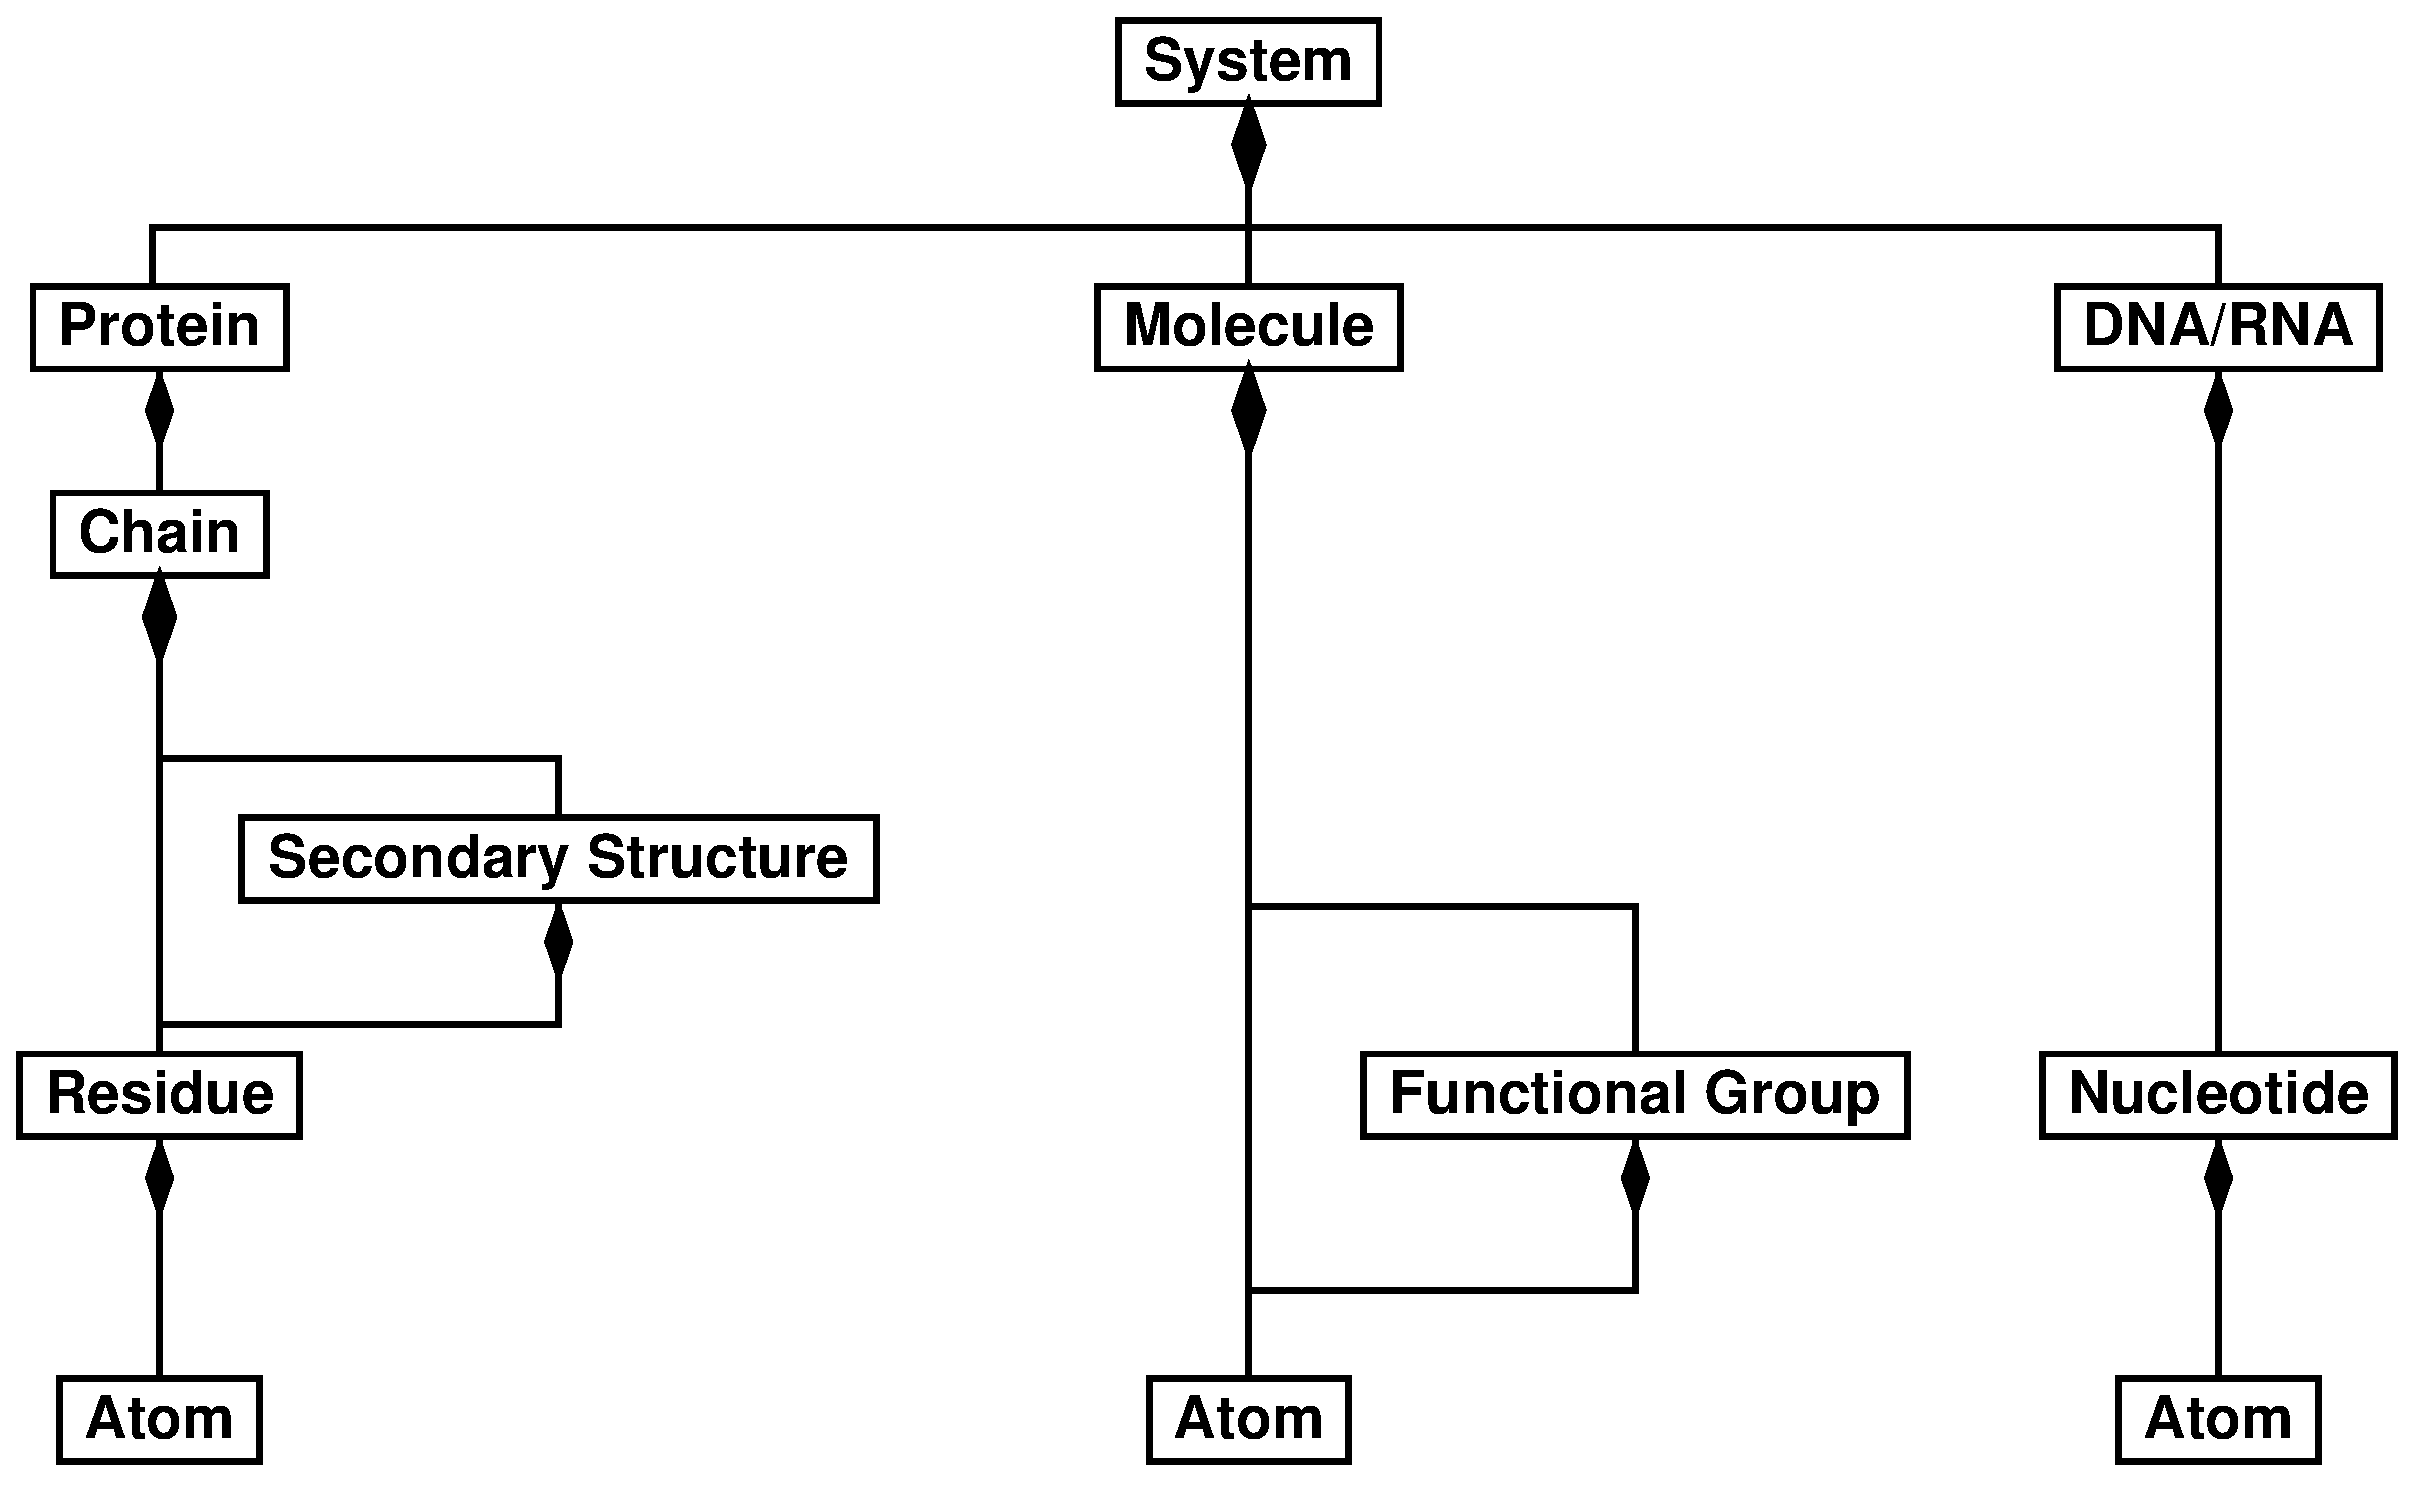
\includegraphics[width=\textwidth]{problem-domain.eps}
  \caption{A model of the biochemical problem domain. BALL tries to model
					these entities as closely as possible with its kernel classes.}
  \label{figure:problem-domain}
\end{figure}

\begin{figure}[tb]
  \centering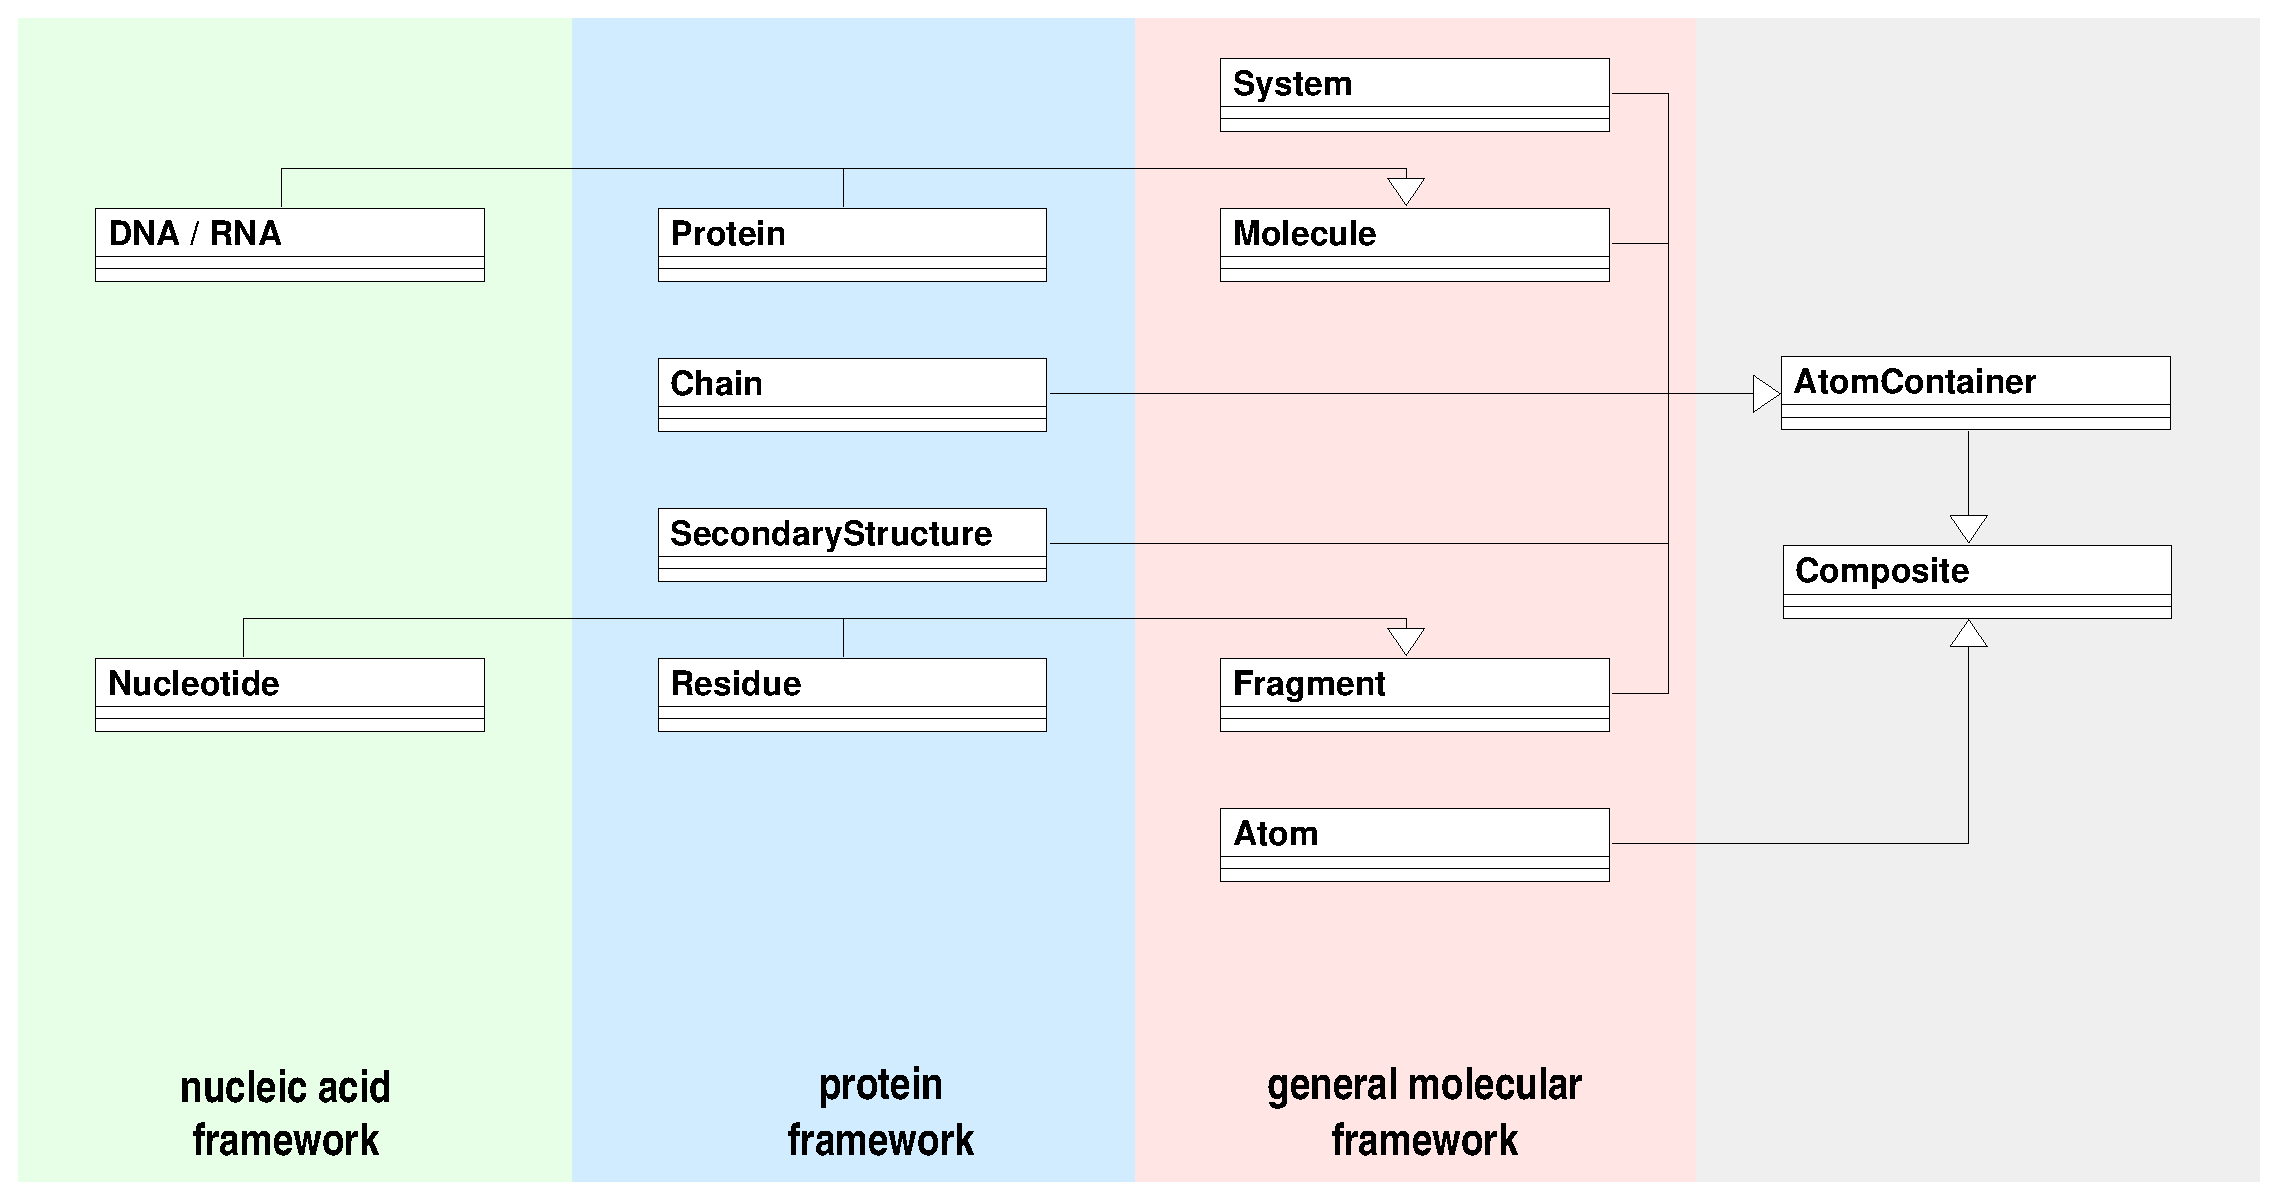
\includegraphics[width=\textwidth]{kernel-data-structures.eps}
  \caption{The BALL kernel classes consist of three main frameworks: the
molecular framework, the protein framework, and the nucleic acid framework.}
  \label{figure:kernel-frameworks}
\end{figure}

\paragraph{The molecular framework} contains the classes \class{System},
\class{Molecule}, \class{Fragment}, \class{Bond}, and \class{Atom}. 
Molecules can contain an arbitrary number of atoms or fragments. A fragment
can be used to define distinct groups in a molecule, \eg functional groups or
charge groups. Fragments can be nested, so you may want to define several
functional groups within one larger fragment in a molecule. The atoms are then
contained in the fragments. In contrast to other systems, the atoms of a
molecule are not necessarily connected to each other (or in graph-theoretical
terms: they do not have to represent a connected component of the graph
formed by atoms and bonds). Systems are nothing but collections of molecules.

\paragraph{The protein framework} is a specialization of the general molecular
framework and describes the structures encountered in proteins. Proteins are
(more or less) molecules, so \class{Protein} is a subclass of \class{Molecule}
and proteins can be handled like molecules and stored along with them in
systems. Proteins can often be decomposed into several chains. These chains in
turn can contain secondary structure elements, which then contain residues.
Residues usually describe the amino acids of a protein. The sequence
information of a protein is encoded implicitly in the order of the tree: it
can be obtained by reading all instances of \class{Residue} in the order they
are contained in a protein. So the protein, the chains, and secondary
structure elements should contain the residues in the correct order, from
N-terminal to C-terminal, if you construct them by hand. The first and last
residue of a chain are considered to be terminal (according to the member
function \member{Residue}{isTerminal}). This is also the reason why a protein
should always contain at least one chain. Secondary structure elements,
defined by \class{SecondaryStructure} are optional. Wherever this information
is known (\eg when read from PDB files), instances of
\class{SecondaryStructure} are created to store it. Each secondary structure
element contains has a property ({\eg helix, $\beta$-sheet) describing its type.

\paragraph{The nucleic acid framework} contains the classes \class{NucleicAcid}
and \class{Nucleotide} and is used to represent structures of nucleic acids.

By deriving all kernel classes from the common base class \class{Composite},
they share all the features implemented there. The following section will
briefly discuss some of these features.

\section{Kernel iterators}
Iteration over kernel data structures is a key concept in BALL.
The BALL kernel iterators are STL-like iterators. Since most BALL kernel
classes are so-called {\em multi-containers}, \ie they can contain different
objects, we cannot use the typical STL {\tt begin()}/{\tt end()} methods.
For example in a protein, you might not only want to iterate over all chains,
but also over all residues or all atoms contained therein. In BALL there
are the methods \member{System}{beginChain()}/\member{System}{endChain()},
\member{System}{beginAtom()}/\member{System}{endAtom()}, and so on for all
kernel classes. Similarly, the iterators are not typedefed within the class,
but are independent classes, because an \class{AtomIterator} could be defined
for any kernel class containing atoms. The only exception from that rule
is \class{Atom::BondIterator}, since an atom is the only container having
bonds. We can use those iterators in an STL-like fashion
\\
\begin{lstlisting}{}
	Molecule m = ...;
	AtomIterator ai;
	for (ai = m.beginAtom(); ai != m.endAtom(); ++ai)
	{
		...
	}
\end{lstlisting}
\noindent but there is also a convenient shorthand, the \method{operator +}
for all iterators. In contrast to STL iterators, BALL iterators are tightly 
bound to their containers and are thus aware of the container's end.
The plus operator returns a boolean value determining the validity of the
operator. It will return {\bf false} as soon as the iterator reaches the
end of the container. So we can rewrite the above code as:
\\
\begin{lstlisting}{}
	Molecule m = ...;
	AtomIterator ai(m.beginAtom());
	for (; +ai; ++ai)
	{
		...
	}
\end{lstlisting}

\noindent 
There exist several variants of the kernel iterators: the standard
forward iterators (\eg \class{AtomIterator}) and reverse iterators
(\class{AtomReverseIterator}). For both, there are also const versions of
these iterators, which are required when iterating over const instances of
kernel classes (\class{AtomConstIterator}, \class{AtomConstReversIterator}).
Iteration is possible for all kernel classes, if they can contain the
respective instances. So it is possible to iterate over all atoms in a
molecule, but it is not possible to iterate over all chains of a residue,
because \class{Residue} does not provide the {\tt beginChain}/{\tt endChain}
methods.

A with the STL, iterators may be dereferenced using both the star operator, and
the arrow operator:\\
\begin{lstlisting}{}
	AtomIterator ai = molecule.beginAtom();
	cout << "first atom: " << (*ai).getName() 
			 << " @ " << ai->getPosition() << std::endl;
\end{lstlisting}

%\section{Selection}???

%\section{Properties}???

%\section{TimeStamps}???


\chapter{VIEW Programming}
\label{chapter:view-programming}
Visualization not only covers the graphical representation of things (\eg
molecules, measurement data, \dots) but also the graphical user interface
(GUI). Both jobs can be done using {\tt VIEW} functionality. Both areas are
discussed in the next few sections. First we will learn how to create
geometric primitives one can use for graphical representations. After that
building a GUI will be shown by creating a user dialog as example.

Let us turn to the graphical representation. In VIEW there are a number of
predefined geometric primitives already available, \eg {\em Sphere}, {\em
Tube} etc. But sometimes a needed primitive may not be available and
therefore must be programmed anew. So now we will show how this can be
achieved. A new primitive, the cross, will be introduced.

\section{How to create a geometric primitive}
\label{section:view_create_a_geometric_primitive}

In this section we want to create a new geometric primitive called 'Cross'.
We define a cross to be a shape that consists of three lines that merge in one
point. Additionally we require all lines to be axis aligned and meet each
other in the middle.

To accomplish this we need three properties for the geometric object: the
float member radius that describes the half length of each line, the class 
\class{Vertex} for the middle point of the geometric primitive and the class 
\class{ColorExtension} which contains methods for changing the color of the
cross. In addition to these classes we need the main base class for
creating a geometric primitive: The \class{GeometricObject} 
implements the interface each geometric shape must have.

The definition of \class{Cross} looks as follows:
\begin{lstlisting}{}
class Cross: 
	public ColorExtension,
	public Vertex,
	public GeometricObject
{
	public:

		Cross() throw();

		virtual ~Cross() throw();
		
		float getRadius() const throw();

		void setRadius(float new_radius) throw();

	protected:
					
		float radius_;
};
\end{lstlisting}

As this object is derived from all the base classes, we only need to implement
a standard constructor, the destructor and the get- and set- methods for 
the radius.
\footnote{The copy constructor and the copy assignment methods
have been omitted because they are not crucial to the implementation of a
primitive.} All additional functionality is provided by inheritance.

We will now have a closer look at the implementation of the drawing method. 
To be able to draw the new geometric object class, we have to add the new
method renderCross\_ to the classes \class{Renderer} and \class{GLRenderer}.

The method Renderer::render\_ defines which drawing methods are called for
which geometric objects. We add the four new lines at the bottom, 
so it recognizes the new class \class{Cross}.

\begin{lstlisting}{}
void Renderer::render_(const GeometricObject* object)
 throw()
{
  if      (RTTI::isKindOf<Sphere>(*object))         
  { 
		renderSphere_(*(const Sphere*) object);
	}
  else if (RTTI::isKindOf<TwoColoredLine>(*object)) 
	{ 
		renderTwoColoredLine_(*(const TwoColoredLine*) object);
	}
  else if (RTTI::isKindOf<Cross>(*object))          
	{ 
		renderCross_(*(const Cross*) object);
	}
  ...
\end{lstlisting}

The method Renderer::renderCross\_(const Cross\& cross)
will be overloaded by derived Renderer classes, so it only
contains a warning, which will appear if we forget to 
implement it in a derived Renderer:

\begin{lstlisting}{}
virtual void renderCross_(const Cross& /* cross */)
	throw() 
{
	Log.error() << "renderCross_ not implemented in derived Renderer class" << std::endl;
}
\end{lstlisting}


The method GLRenderer::renderCross\_(const Cross\& cross)
does the actual rendering, so we use OpenGL code here:

\begin{lstlisting}{}
void GLRenderer::renderCross_(const Cross& cross)
	throw() 
{
	glPushMatrix();
	
	// if cross is selected, use the selection color,
	// otherwise use its own color. (method from GLRenderer)
	setColor4ub_(cross);  
	
	// move to the position of the cross (method from GLRenderer)
	translateVector3_(sphere.getVertex());
	
	// OpenGL code for rendering the cross.
	glBegin(GL_LINES);
	glVertex3f((GLfloat)(getVertex().x - cross.getRadius()),
						 (GLfloat)(getVertex().y),
						 (GLfloat)(getVertex().z));
	glVertex3f((GLfloat)(getVertex().x + cross.getRadius()),
						 (GLfloat)(getVertex().y),
						 (GLfloat)(getVertex().z));

	glVertex3f((GLfloat)(getVertex().x),
						 (GLfloat)(getVertex().y - cross.getRadius()),
						 (GLfloat)(getVertex().z));
	glVertex3f((GLfloat)(getVertex().x),
						 (GLfloat)(getVertex().y + cross.getRadius()),
						 (GLfloat)(getVertex().z));

	glVertex3f((GLfloat)(getVertex().x),
						 (GLfloat)(getVertex().y),
						 (GLfloat)(getVertex().z - cross.getRadius()));
	glVertex3f((GLfloat)(getVertex().x),
						 (GLfloat)(getVertex().y),
						 (GLfloat)(getVertex().z + cross.getRadius()));
	glEnd();

	glPopMatrix();
}
\end{lstlisting}


\section{Construction of a dialog}
\label{section:view_construction_of_a_dialog}

A crucial step in implementing an application is the programming of dialogs or
widgets, their interaction with other widgets and the integration into the
main application. We will now discuss the creation of a dialog that will have
all the above properties. A widget can be created in a similar manner, by
exchanging the \class{QDialog} base class with the \class{QWidget} class. That
should do the trick.

The construction of a dialog/widget is somewhat complicated because of the
many actions it can perform. A dialog can have menu entries in the main
application (derived from the \class{MainControl}) and can react to messages
sent from other dialogs/widgets (see \class{Message} and
\class{ModularWidget}). We want to create a dialog which has both of the
above properties. As an example we choose the \class{LabelDialog}, which already
exists in the VIEW library. This dialog can add Labels to the visualisation of
molecules.
We created the GUI of the dialog with the program "QT Designer" which is part
of every QT-package. This has the advantage, that the creation of the GUI takes
less time and the layout can be changed with much less effort. 
The result of the "designer" program is a .ui file, which the program "uic"
from the QT-library transforms to source files. We derive from the class
LabelDialogData, that is defined in these sources.

The menu entry "Add Label" for our dialog will toggle the visibility of the dialog itself.
The color for the labels will be written to
and read from the \class{INIFile}, which the main application keeps. The
\class{Message} that should trigger some effect will be the message 
\class{ControlSelectionMessage} that is sent by the class \class{MolecularControl} 
whenever the selection changes. To accomlish all these things we have to 
override certain methods.

First we have a look to the header file of our dialog (includes are omitted).
See \class{ModularWidget} for information about the various methods that must
be overridden.

\begin{lstlisting}{}

class LabelDialog : 
	public LabelDialogData,
	public ModularWidget
{
	Q_OBJECT
	
	// needed for getInstance() and for Python Interface
	BALL_EMBEDDABLE(LabelDialog,ModularWidget)
		
	public:
	
	LabelDialog(QWidget *parent = NULL, const char *name = NULL )
		throw();

	virtual ~LabelDialog()
		throw();
					
	virtual void onNotify(Message *message)
		throw();
					
	virtual void fetchPreferences(INIFile &inifile)
		throw();
	
	virtual void writePreferences(INIFile &inifile)
		throw();
		
	virtual void initializeWidget(MainControl& main_control)
		throw();
	
	virtual void finalizeWidget(MainControl& main_control)
		throw();
				
	public slots:

	void show();

	protected slots:
					
	virtual void accept();
	virtual void editColor();

private:
	
	int id_;
	
	ColorRGBA custom_color_;
	List<Composite*> selection_;
};
\end{lstlisting}

Now we discuss the implementation. Before we handle the initialization,
update and the removal of the menu entries let's have a look to the
implementation of the constructor. First we set the caption of this dialog
and register it as a modular widget. This action is very important because it
creates the internal mechanism that connects all widgets with each other. If
you create your own dialogs/widgets which have to react to messages always make 
sure this method is called.

\begin{lstlisting}{}
LabelDialog::LabelDialog(QWidget* parent, const char* name)
	throw()
	:	LabelDialogData( parent, name ),
		ModularWidget(name)
{
	setCaption("Add Label");

	// register the widget with the MainControl
	ModularWidget::registerWidget(this);

	hide();
}
\end{lstlisting}

The next method creates the menu entry for our dialog and connects it to a slot
that will open our dialog. First we create the menu {\em DISPLAY} if it is not
already created and set the flag {\em checkable} to assure that all entries
can have a check flag.
Then we create the menu entry {\em Add Label} in the menu {\em DISPLAY} and
connect it with the slot LabelDialog::show(), which is provided by the class QWidget. 
The id we get from this method is stored in the variable id\_. We need this
id to check the menu entry if this dialog is open.

\begin{lstlisting}{}
void LabelDialog::initializeWidget(MainControl& main_control)
	throw()
{
	main_control.initPopupMenu(MainControl::DISPLAY)->setCheckable(true);

	id_ = main_control.insertMenuEntry(MainControl::DISPLAY, "Add &Label", this,
																		 SLOT(show()), CTRL+Key_L, -1,
																		 "Add a label for selected molecular objects");   
}

\end{lstlisting}

Finally, if the dialog is to be destroyed the menu entry will be removed from
the main application (derived from {\em MainControl}).
\begin{lstlisting}{}
void LabelDialog::finalizeWidget(MainControl& main_control)
	throw()
{
	main_control.removeMenuEntry(MainControl::DISPLAY, "Add &Label", this,
															 SLOT(show()), CTRL+Key_L);   
}
\end{lstlisting}

In the above methods it as also possible to do other initialization or menu handling stuff.
It is also possible to add, update and remove more menu entries (for each menu entry
there must be a slot to be connected to).


The next methods we will discuss are the methods responsible for reading and
writing the contents of this widget into the \class{INIFile}. First we look at the
method responsible form reading the preferences.
If the \class{INIFile} has the section {\tt WINDOWS} and the key {\tt Label::customcolor} then
we read the contents of this key and convert it to a color which we store in
\member{custom\_color\_}{} (see \class{ColorRGBA}). 
Additionally we assign the color to the label to be displayed in the widget.

\begin{lstlisting}{}
void LabelDialog::fetchPreferences(INIFile& inifile)
	throw()
{
	if (inifile.hasEntry("WINDOWS", "Label::customcolor"))
	{
		custom_color_.set(inifile.getValue("WINDOWS", "Label::customcolor"));
		color_sample_->setBackgroundColor(custom_color_.getQColor());
	}
	else
	{
		custom_color_.set(ColorRGBA(1.,1.,0.,1.));
		color_sample_->setBackgroundColor(custom_color_.getQColor());
	}			
}
\end{lstlisting}

To write the preferences to the inifile we override this method.

\begin{lstlisting}{}
void LabelDialog::writePreferences(INIFile& inifile)
	throw()
{
	inifile.insertValue("WINDOWS", "Label::customcolor", custom_color_);
}
\end{lstlisting}

{\em Note:} It is important that the section {\tt WINDOWS} is
already inserted into the inifile, else the inifile will not store the color.
See \class{INIFile} for further information.

The last method of the preferences tab widget is the method editColor  that
is called if the edit button is pressed.
First we call the dialog \class{QColorDialog} where we can change the color.
If this dialog was exited by pressing the ok button we transfer the color into
the color label. Then we store it in the variable custom\_color\_.

\begin{lstlisting}{}
void LabelDialog::editColor()
{
	color_sample_->setBackgroundColor(
			QColorDialog::getColor(color_sample_->backgroundColor()));
	QColor qcolor = color_sample_->backgroundColor();

	custom_color_.set(qcolor);
	update();
}
\end{lstlisting}

The slot accept is connected to the apply button and will add the label
to the visualisation of the selected molecular objects:
\begin{lstlisting}{}
void LabelDialog::accept()
{
	// no selection present => return
	if (selection_.empty()) return;

	// calculate the geometric center for the selection
	GeometricCenterProcessor center_processor;
	
	// center to which the label will be attached
	Vector3 center;

	// process all objects in the selection list
	List<Composite*>::Iterator list_it = selection_.begin();
	for (; list_it != selection_.end(); ++list_it)
	{
		(*list_it)->apply(center_processor);
		center += center_processor.getCenter();
	}

	center /= selection_.size();

	// create a new Label 
	Label* label = new Label;
	label->setText(label_edit_->text().ascii());
	label->setColor(custom_color_);
	label->setVertex(center);

	// create a new Representation
	Representation* rep = getMainControl()->
				getPrimitiveManager().createRepresentation();
	rep->insert(*label);
	rep->setProperty(Representation::PROPERTY__ALWAYS_FRONT);
	rep->setModelType(MODEL_LABEL);

	// create and send a RepresentationMessage to inform the Scene and
	// update the GeometricControl
	RepresentationMessage* rm = new RepresentationMessage;
	rm->setRepresentation(*rep);
	rm->setType(RepresentationMessage::ADD);
	notify_(rm);
	
	setStatusbarText("Label added.");
}
\end{lstlisting}

The only thing that still must be implemented is the mechanism that handles
any messages received from our dialog. This is done in the method
onNotify. 
We perform a runtime type identification of the received message and react only if the message is of
type \class{SelectionMessage}.
We enable the apply button in our dialog if the selection list contains any
elements. Otherwise we disable it.

\begin{lstlisting}{}
void LabelDialog::onNotify(Message *message)
	throw()
{
	// selection => store last selection for later processing
	if (RTTI::isKindOf<ControlSelectionMessage>(*message))
	{
		ControlSelectionMessage* selection = 
			RTTI::castTo<ControlSelectionMessage>(*message);
		selection_ = selection->getSelection();
	}

	// disable apply button, if selection is empty
	apply_button_->setEnabled(!selection_.empty());
	menuBar()->setItemEnabled(id_, !selection_.empty());
}
\end{lstlisting}


Now we are finished with the construction of this dialog. It can be added to
the main application by creating it with a pointer to the application ({\em
MainControl}) as parent.



\chapter{Python Extensions}
\label{chapter:python}
\section{Overview}
Python is an object-oriented scripting language\cite{Python} that is well
suited both as a language for embedding scripts into BALL application and as a
rapid prototyping language using the underlying BALL objects.
BALL provides Python bindings for most of its classes in order to allow Rapid
Methodology Development (RMD). Some of the functionality BALL provides (\eg
template classes, iterators) are unavailable due to the fundamental differences 
between the two languages. However, the majority of the classes is available and
workarounds exist for some of the template- and iterator-related problems.

The current Python support is not yet fully tested and debugged, therefore it
is disabled by default. If you can live with
this and think it is still a useful feature worth testing out, please read on,
otherwise pretend it doesn't exist. The remainder of this section assumes that
you are somewhat familiar with the most important language concepts of Python.

BALL relies on SIP \cite{SIP} (version 4.3.1 or above) to translate its class
headers semi-automatically into python wrapper classes. For each \CPP class
SIP creates a subclass defining the Python interface and a Python class
using that \CPP interface class. The Python class has the same name as the
\CPP class, so porting code from \CPP to Python (and vice versa) gets trivial.
The \CPP code 

\begin{lstlisting}{}
	System S;
	HINFile f("test.hin");
	f >> S;
\end{lstlisting}

\noindent
translates to the Python code

\begin{lstlisting}{}
	S = System()
	f = HINFile("test.hin")
	f >> S;
\end{lstlisting}

\noindent
In this example, the main difference lies in the way \CPP and Python handle
constructors. Another important difference concerns iterators. The STL-like
kernel iterators of BALL map to a set of functions (called extractors). An
extractor traverses the whole container and creates a Python sequence object
from it. Instead of having an \class{AtomIterator} iterating over all atoms of
a residue

\begin{lstlisting}{}
	AtomIterator ai = residue.beginAtom();
	for (; +ai; ++ai)
	{
		std::cout << ai->getName() << std::endl;
	}
\end{lstlisting}
\noindent you would use the \function{atoms} extractor to create a sequence
object containing all objects of the residue in Python:

\begin{lstlisting}{}
	for atom in atoms(residue):
		print atom.getName()
\end{lstlisting}

\noindent For the template problem, we pre-instantiated some of the 
commonly used instances, \eg \class{UnaryProcessor<Atom>} maps to the 
\class{AtomProcessor} class and classes derived from it in Python.

The BALLView application contains an interactive interpreter window
if BALL was compiled with Python support. You can even access the
data structures of the viewer from there. Assuming that you are
currently displaying a structure in the viewer, you can retrieve a
reference to the first system displayed through the somewhat cryptic
command 
\\
{\tt system = MainControl::getInstance(0)\\
.getCompositeManager().getComposites()[0]}.
Since this is not very convenient, we added a Python startup script,
that will always be run when BALLView starts up. It can be found
under BALL/data/startup.py. By using one of the methods defined in this file,
it is possible to obtain the first System by simply calling \\
{\tt system = getSystem(0)}.
This is pretty useful for extracting properties from the loaded molecules
and other datasets you are
currently displaying, but very deadly if you start modifying internals
of the viewer. You also should not try to destroy those objects in the
viewer, or you will be rewarded with a core dump: there is not yet
internal reference counting on the BALL side, so Python's reference
counting is nearly always wrong.
		

\section{Known bugs}
\begin{itemize}
	\item No documentation yet
	\item No unit tests yet
	\item As mentioned above, problems with reference counting.
	\item Python support requires the visualization support for some rather
				arcane internal reason we won't disclose here.
	\item {\tt configure} does not yet identify SIP and its libraries
				automatically
\end{itemize}

\section{Installation}

Donwload, configure, and install a recent version (4.3.1 or above) of SIP from 
\URL{http://www.riverbankcomputing.co.uk/sip/}. It is important to compile BALL 
with the same \CPP compiler you compiled SIP and QT with. You can then enable the Python support of BALL
by specifying the option \mbox{"\option{--with-python=<path>}"}, where
{\tt path} should point to the executable of an installed Python (version 2.3
preferred). You will also have to specify the path to the SIP executable, its
headers, and its library ({\tt libsip.a|so}). Adding these four options might
look something like this on your system:

\begin{lstlisting}{}
	./configure \
		--with-python=/opt/bin/python2.3\
		--with-sip=/opt/bin/sip\
		--with-sip-incl=/opt/include/sip\
		--with-sip-lib=/opt/lib
\end{lstlisting}

\noindent
After configuring and building BALL, you should then change to {\tt
BALL/source/PYTHON/EXTENSIONS}. Here, you will have to run

\begin{lstlisting}{}
	make sip
	make depend
	make
	make install
\end{lstlisting}

\noindent
in order to build the Python bindings, which are then installed to {\tt
BALL/lib/<platform>}. 
You can then execute the {\tt pyball} script in {\tt
BALL/source/PYTHON/EXTENSIONS} to get an interactive Python shell with the
BALL bindings or just start the Python interpreter and import the BALL
bindings through

\begin{lstlisting}{}
	from BALL import *
\end{lstlisting}

\noindent
Note, that you have to add the directory where the bindings are installed to
Python's module search path ({\tt sys.path}).


\chapter{FAQ}
\label{chapter:faq}
\newpage
\noindent
{\it An up-to-date and searchable version of this FAQ is available at our website:\\
\FAQURL{http://www.ball-project.org/Support/FAQ}}\\
\hspace{1mm}
\rule{\textwidth}{0.1pt}
\hspace{3mm}
\FAQCategory{Documentation}
\FAQquestion{Are there Research reports available?}
\FAQanswer{Yes. Publications and research reports on BALL are listed on our website: 
\FAQURL{http://www.ball-project.org}
}
\FAQquestion{How do I use BALLView?}
\FAQanswer{Take a look at the builtin BALLView Tutorial or on the documentation at http://www.ball-project.org/Documentation or under BALL/doc/BALLView}
\FAQCategory{Installation}
\FAQquestion{Will BALL run on my hardware/with my compiler?}
\FAQanswer{An up-to-date list of all supported platforms can be found on the BALL website at 
\FAQURL{http://www.ball-project.org/Support/FAQ/Platforms}
}
\FAQCategory{License}
\FAQquestion{Under what kind of license is BALL available?}
\FAQanswer{
	BALL is mostly being distributed under the Lesser GNU Public License (LGPL). Parts of BALL (BALLView) are under the GNU Public License (GPL).
}



\newpage
\addtocontents{toc}{\protect\contentsline{chapter}{Index}{\thepage}}
\printindex
\renewcommand{\bibname}{References}
\addtocontents{toc}{\protect\contentsline{chapter}{References}{\thepage}}
\bibliographystyle{abbrv}
\bibliography{tutorial}

\end{document}
